%%
%% This is file `sample-sigconf.tex',
%% generated with the docstrip utility.
%%
%% The original source files were:
%%
%% samples.dtx  (with options: `all,proceedings,bibtex,sigconf')
%% 
%% IMPORTANT NOTICE:
%% 
%% For the copyright see the source file.
%% 
%% Any modified versions of this file must be renamed
%% with new filenames distinct from sample-sigconf.tex.
%% 
%% For distribution of the original source see the terms
%% for copying and modification in the file samples.dtx.
%% 
%% This generated file may be distributed as long as the
%% original source files, as listed above, are part of the
%% same distribution. (The sources need not necessarily be
%% in the same archive or directory.)
%%
%%
%% Commands for TeXCount
%TC:macro \cite [option:text,text]
%TC:macro \citep [option:text,text]
%TC:macro \citet [option:text,text]
%TC:envir table 0 1
%TC:envir table* 0 1
%TC:envir tabular [ignore] word
%TC:envir displaymath 0 word
%TC:envir math 0 word
%TC:envir comment 0 0
%%
%% The first command in your LaTeX source must be the \documentclass
%% command.
%%
%% For submission and review of your manuscript please change the
%% command to \documentclass[manuscript, screen, review]{acmart}.
%%
%% When submitting camera ready or to TAPS, please change the command
%% to \documentclass[sigconf]{acmart} or whichever template is required
%% for your publication.
%%
%%
\documentclass[sigconf]{acmart}
\settopmatter{printacmref=false} 

% Remove copyright footnote
%\renewcommand\footnotetextcopyrightpermission[1]{}

% Use plain page style to remove header/footer info
%\pagestyle{plain}


\usepackage{tikz}
\usepackage{pgfplots}
\usepackage{subfig}
\usetikzlibrary{plotmarks}
\usepackage{amsmath}
\usepackage{filecontents}
\usepackage{float}
\usepackage{soul}
\usepackage{verbatim}


\pgfplotsset{
      % #1: index in the group(0,1,2,\ldots)
      % #2: number of plots of that group
  bar group size/.style 2 args={
    /pgf/bar shift={%
                                  % total width = n*w + (n-1)*skip
                                  % -> subtract half for centering
      -0.5*(#2*\pgfplotbarwidth + (#2-1)*\pgfkeysvalueof{/pgfplots/bar group skip})  +
                                                  % the '0.5*w' is for centering
      (.5+#1)*\pgfplotbarwidth + #1*\pgfkeysvalueof{/pgfplots/bar group skip}},%
    },
    bar group skip/.initial=2pt,
    tbb/.style={black, fill=black!30, pattern=crosshatch},%
    tbbpatch/.style={black, fill=yellow!30, pattern=north east lines},%
    ff/.style={black, fill=black},%
    %tbbpatch/.style={red,fill=red!30!white,mark=none},%
    %ff/.style={brown!60!black,fill=brown!30!white,mark=none},%
  }



\pgfplotsset{qatime/.style={%
  ytick={0, 20, 40, 60, 80, 100},
  tick label style={font=\normalsize},
  label style={font=\normalsize},
  ylabel= {累积分布函数(\%)},
  xlabel = {时间(小时)},
  ymin=0,
  ymax=165,
  %ymax=110,
%  xmax = 12,
  scale only axis,
  width=0.9\textwidth,
  height=0.6\textwidth,
  legend style={legend pos=north west, font=\normalsize},
  xmin=0.01,
  every axis/.append style={font=\normalsize}
}
}
\pgfplotsset{recdf/.style={%
  tick label style={font=\normalsize},
  label style={font=\normalsize},
  ylabel= {累积分布函数(\%)},
  %ylabel= {Ratio(\%)},
  xlabel = {时间(小时)},
  ymin=0,
  ytick={0, 20, 40, 60, 80, 100},
  ymax=180,
  scale only axis,
  width=0.9\textwidth,
  height=0.6\textwidth,
  legend style={legend pos=north west, font=\normalsize},
  xmin=0,
  every axis/.append style={font=\normalsize}
}
}

  \pgfplotsset{avgtime/.style={%
    legend style={
      at={(0.5,0.98)},
      legend columns=3,
      font=\normalsize,
    anchor=north},
    ybar,
    xtick pos = left,
    bar width=9pt,
    ymin=0,
    ymax=110,
    xmin=0.3,
    scale only axis,
    ytick={0, 20, 40, 60, 80, 100},
    xticklabels={\normalsize {\bh{.}}, \bh{.}, \footnotesize{\bh{TM}}, \footnotesize{\bh{CQ}}, \footnotesize{\bh{CP}}, \footnotesize{\bh{ST}}, \footnotesize{\bh{OM}}, \footnotesize{\bh{WT}}, \footnotesize{\bh{PP}}, \footnotesize{\bh{DP}}, \footnotesize{\bh{MX}},\footnotesize{\bh{TR}}},
    ylabel style={align=center},
    ylabel={{时间(分钟)}},
    xlabel=\empty,
    width=1.3\textwidth,
    height=0.4\textwidth,
    every axis/.append style={font=\normalsize},
    after end axis/.code={
    \draw [decorate,decoration={brace,mirror,raise=15}] (axis cs:0.5,0) --
    (axis cs:5.4,0) node [midway,below=15] {\normalsize 解决编译错误};
    \draw [decorate,decoration={brace,mirror,raise=15}] (axis cs:5.6,0) --
    (axis cs:8.4,0) node [midway,below=15] {\normalsize 解决运行时错误};
    \draw [decorate,decoration={brace,mirror,raise=15}] (axis cs:8.6,0) --
    (axis cs:10.5,0) node [midway,below=15] {\normalsize 并行编程};
                          }
  }}
\pgfplotsset{speedupbar/.style={%
  legend style = {
    cells={anchor=east},
    legend pos=north west,
    font=\normalsize,
    legend columns=2,
  },
  xticklabels={\normalsize {\bench{KM}}, \normalsize {\bench{CA}},
    \normalsize{\bench{LU}},
    \normalsize{\bench{QD}},
    \normalsize{\bench{FB}},
    \normalsize{\bench{QS}}, \normalsize{\bench{TS}},
    \normalsize{\bench{NQ}}},
  scale only axis,
  xtick=data,
  ybar,
  ytick = {0, 1, 2, 3, 4, 5, 6, 7, 8},
  ylabel={加速比},
  ymin=0,
  ymax=8.7,
  width = .75\textwidth,
  height= .45\textwidth,
  bar width = 10pt,
  xtick pos = left,
  every axis/.append style={font=\normalsize},
}}

\pgfplotsset{scalline/.style={%
  legend style = {
    cells={anchor=east},
    legend pos=north west,
    font=\normalsize,
    legend columns=2,
  },
  scale only axis,
  xtick=data,
  ytick = {0, 1, 2, 3, 4, 5, 6, 7, 8},
  ymin = 0,
  ymax = 8,
  xmax = 8,
  xtick pos = left,
  xlabel = {处理器个数},
  ylabel = {加速度比},
  width = .75\textwidth,
  height= .45\textwidth,
  grid,
  every axis/.append style={font=\normalsize},
}}

\pgfplotsset{microvarbar/.style={%
  yticklabel={\pgfmathprintnumber{\tick}},
       legend style={
          at={(0.5,0.98)},
          legend columns=1,
          font=\footnotesize,
          anchor=north},
        ybar,
        bar width=9pt,
        ymin=0,
        xmax=4.4,
        xmin=0.5,
        scale only axis,
        ylabel={\footnotesize{Variance ($\log_{10}$)}},
        xlabel={\footnotesize{\# of lock}},
        xtick=data,
        %xtick={3e12, e13, 3e13},
        every axis y label/.append style={
          yshift=-8pt,
        },
        width=0.75\textwidth,
        height=0.6\textwidth,
        every axis/.append style={font=\footnotesize}
}}

\pgfplotsset{mhtime/.style={%
        tick label style={font=\footnotesize},
        label style={font=\footnotesize},
        xlabel= {\footnotesize{Ratio of locks' duration.}},
        ylabel= {\footnotesize{Speedup}},
        ymin=1,
        ymax=4,
        width=\textwidth,
        height=0.86\textwidth,
        xmin=0,
        xmax=100,
        every axis y label/.append style={
          yshift=-12pt,
        },
        every axis/.append style={font=\footnotesize}}
}

\pgfplotsset{allbench/.style={%
       legend style={
          at={(0.5,0.98)},
          legend columns=3,
          font=\footnotesize,
          anchor=north},
        ybar,
        bar width=6pt,
        ymin=0.7,
        ymax=1.3,
        xmin=0.5,
        xmax=6.8,
        scale only axis,
        xticklabels={\bench{BQ}, \bench{VN}, \bench{SSCA}, \bench{CA},
          \bench{SC}, \bench{QS}},
        ylabel style={text width = .16\textwidth, align=center},
        ylabel={Runtime (normalized)},
        xlabel=\empty,
        xtick=data,
        every axis y label/.append style={
          yshift=-1pt,
        },
        x tick label style={rotate=45,anchor=east},
        ytick = {0.6, 0.7, 0.8, 0.9, 1.0, 1.1},
        width=0.95\textwidth,
        height=0.24\textwidth,
        every axis/.append style={font=\footnotesize}
}}



\pgfplotsset{tcdf2/.style={%
  tick label style={font=\normal},
  label style={font=\normal},
  ylabel= {累积分布函数(\%)},
  %    ylabel= {Ratio(\%)},
  xlabel = {时间(分钟)},
  ymin=0,
  ytick={0, 20, 40, 60, 80, 100},
  ymax=105,
  scale only axis,
  width=0.25\textwidth,
  height=0.3\textwidth,
  legend style={legend pos=south east, font=\normal},
  xmin=0,
  every axis/.append style={font=\normal}
}
  }
  \pgfplotsset{tcdf3/.style={%
    tick label style={font=\normal},
    label style={font=\normal},
    ylabel= {累积分布函数(\%)},
    %ylabel= {Ratio(\%)},
    xlabel = {时间(分钟)},
    ymin=0,
    ytick={0, 20, 40, 60, 80, 100},
    ymax=130,
    scale only axis,
    width=0.25\textwidth,
    height=0.3\textwidth,
    legend style={legend pos=north east, font=\normal},
    xmin=0,
    every axis/.append style={font=\normal}
  }
}


\pgfplotsset{bqvarbar/.style={%
        %y tick label style={/pgf/number format/.cd,sci precision=5},
  yticklabel={\pgfmathprintnumber{\tick}},
       legend style={
         legend pos = north west,
          legend columns=1,
          font=\footnotesize,
          },
        ybar,
        bar width=9pt,
        ymin=0,
        ymax = 200000,
        xmin=0.7,
        xmax = 2.3,
        scale only axis,
        ylabel={\footnotesize{方差($\log_{10}$)}},
        xlabel={\footnotesize{锁的个数}},
        xtick=data,
        every axis y label/.append style={
          yshift=-16pt,
        },
        width = 0.4\textwidth,
        height=0.15\textwidth,
        every axis/.append style={font=\footnotesize}
}}

\pgfplotsset{vnvarbar/.style={%
  yticklabel={\pgfmathprintnumber{\tick}},
       legend style={
         legend pos = north west,
          legend columns=1,
          font=\footnotesize,
          },
        ybar,
        bar width=9pt,
        ymin=0,
        ymax=1e12,
        xmin=0.5,
        xmax = 4.5,
        scale only axis,
        ylabel={\footnotesize{Variance ($\log_{10}$)}},
        xlabel={\footnotesize{\# of lock}},
        xtick=data,
        every axis y label/.append style={
          yshift=-16pt,
        },
        width = 0.4\textwidth,
        height=0.15\textwidth,
        every axis/.append style={font=\footnotesize}
}}

\pgfplotsset{alllb/.style={%
       legend style={
          legend columns=1,
          font=\footnotesize,
          legend pos=north west},
        ybar,
        bar width=7pt,
        ymin=60,
        ymax=100,
        xmin=0.5,
        xmax=6.8,
        scale only axis,
        xticklabels={\bench{BQ}, \bench{VN}, \bench{SSCA}, \bench{CA}, \bench{SC}, \bench{QS}},
    ylabel={\footnotesize{负载均衡(\%)}},
        xlabel=\empty,
        xtick=data,
        x tick label style={rotate=45,anchor=east},
        width=0.75\textwidth,
        height=0.36\textwidth,
        every axis/.append style={font=\footnotesize}
}}


\pgfplotsset{bposs1/.style={%
    xlabel={锁的个数 ($L$)},
    tick label style={font=\footnotesize},
    label style={font=\footnotesize},
    ylabel={\footnotesize{时间}},
    scale only axis,
    width=0.36\textwidth,
    height=0.36\textwidth,
    grid=major,
    ymin=0,
    xmin=0,
    every axis y label/.append style={
      yshift=-20pt,
    },
    every axis/.append style={font=\footnotesize}}}

\pgfplotsset{bposs2/.style={%
    xlabel={锁的个数 ($L$)},
    tick label style={font=\footnotesize},
    label style={font=\footnotesize},
    ylabel={\footnotesize{时间}},
    %ylabel=\empty,
    scale only axis,
    width=0.36\textwidth,
    height=0.36\textwidth,
    grid=major,
    ymin=0,
    xmin=0,
    every axis y label/.append style={
      yshift=-15pt,
    },
    every axis/.append style={font=\footnotesize}
  }}

\pgfplotsset{bposs3/.style={%
    xlabel={锁的个数 ($L$)},
    tick label style={font=\footnotesize},
    label style={font=\footnotesize},
    ylabel={\footnotesize{时间}},
    %ylabel=\empty,
    scale only axis,
    width=0.36\textwidth,
    height=0.36\textwidth,
    grid=major,
    ymin=0,
    xmin=0,
    every axis y label/.append style={
      yshift=-5pt,
    },
    every axis/.append style={font=\footnotesize}
  }}
\pgfplotsset{singlelb/.style={%
    tick label style={font=\footnotesize},
    label style={font=\footnotesize},
    ylabel= {\footnotesize{Load balancing(\%)}},
    grid=major,
    ymin=40,
    ymax=100,
    scale only axis,
    width=0.3\textwidth,
    height=0.33\textwidth,
    xmin=0,
    every axis y label/.append style={
      yshift=-12pt,
    },
    every axis/.append style={font=\footnotesize}}}

\pgfplotsset{cpuusage1/.style={%
    tick label style={font=\footnotesize},
    label style={font=\footnotesize},
    ylabel= {\footnotesize{Utilization(\%)}},
    grid=major,
    ymin=40,
    ymax=105,
    scale only axis,
    width=0.15\textwidth,
    height=0.15\textwidth,
    xmin=0,
    every axis y label/.append style={
      yshift=-12pt,
    },
    ytick={40, 60, ..., 120},
    every axis/.append style={font=\footnotesize}}}

\pgfplotsset{cpuusage2/.style={%
    tick label style={font=\footnotesize},
    label style={font=\footnotesize},
    ylabel={\footnotesize{CPU利用率(\%)}},
    grid=major,
    ymin=40,
    ymax=105,
    scale only axis,
    width=0.35\textwidth,
    height=0.35\textwidth,
    xmin=0,
    every axis y label/.append style={
      yshift=-12pt,
    },
    ytick={40, 60, ..., 120},
    every axis/.append style={font=\footnotesize}
  }}



\pgfplotsset{lockusage/.style={%
    legend style={
      at={(0.5,0.98)},
      legend columns=2,
      font=\footnotesize,
      anchor=north},
    ybar stacked,
    scale only axis,
    ylabel={\footnotesize{\# of acquired locks (million)}},
    xlabel={\footnotesize{\# thread}},
    symbolic x coords={{0},{1}, {2}, {3}},
    ymin=0,
    ymax= 15,
    xtick=data,
    every axis y label/.append style={
      yshift=-15pt,
    },
    y tick label/.append style={/pgf/number format/.cd,%
      scaled y ticks = false,
      set thousands separator={$*$},
      fixed,
    },
    width=0.15\textwidth,
    height=0.25\textwidth,
    every axis/.append style={font=\footnotesize}
  }}

\pgfplotsset{benchlockusage/.style={%
    legend style={
      at={(0.5,0.98)},
      legend columns=2,
      font=\footnotesize,
      anchor=north},
    ybar stacked,
    scale only axis,
    ylabel={\footnotesize{\# of acquired locks (million)}},
    xlabel={\footnotesize{\# thread}},
    %symbolic x coords={{0},{1}, {2}, {3}, {4}, {5}, {6}, {7}},
    ymin=0,
    %ymax= 15,
    xtick=data,
    every axis y label/.append style={
      yshift=-15pt,
    },
    y tick label/.append style={/pgf/number format/.cd,%
      scaled y ticks = false,
      set thousands separator={$*$},
      fixed,
    },
    %width=0.15\textwidth,
    %height=0.25\textwidth,
    every axis/.append style={font=\footnotesize}
  }}
\pgfplotsset{mainbench/.style={%
    ybar,
    bar width=5pt,
    ymin=0,
    xmin=0,
    scale only axis,
    legend style={legend pos=outer north east,font=\footnotesize},
    ylabel={\footnotesize{Runtime (s)}},
    xlabel={\footnotesize{\# of threads}},
    xtick=data,
    width=0.85\textwidth,
    height=0.75\textwidth,
    every axis/.append style={font=\footnotesize}
  }}

\pgfplotsset{alllb/.style={%
    legend style={
      legend columns=1,
      font=\footnotesize,
      legend pos=north west},
    ybar,
    bar width=7pt,
    ymin=60,
    ymax=100,
    xmin=0.5,
    xmax=6.8,
    scale only axis,
    xticklabels={\bench{BQ}, \bench{VN}, \bench{SSCA}, \bench{CA}, \bench{SC}, \bench{QS}},
    ylabel={\footnotesize{负载均衡(\%)}},
    xlabel=\empty,
    xtick=data,
    x tick label style={rotate=45,anchor=east},
    width=0.75\textwidth,
    height=0.36\textwidth,
    every axis/.append style={font=\footnotesize}
  }}

\pgfplotsset{cachemiss/.style={%
    legend style={
      legend columns=1,
      font=\footnotesize,
      anchor=north east},
    ybar,
    bar width=7pt,
    ymin=0,
    ymax=45,
    xmin=0.5,
    xmax=6.8,
    ytick={0, 10, 20, 30, 40},
    scale only axis,
    xticklabels={\bench{BQ}, \bench{VN}, \bench{SSCA}, \bench{CA}, \bench{SC}, \bench{QS}},
    ylabel={\footnotesize{缓存缺失率(\%)}},
    xlabel=\empty,
    xtick=data,
    every axis y label/.append style={
      yshift=-16pt,
    },
    x tick label style={rotate=45,anchor=east},
    width=0.95\textwidth,
    height=0.6\textwidth,
    every axis/.append style={font=\footnotesize}
  }}

\pgfplotsset{allbench/.style={%
    legend style={
      at={(0.5,0.98)},
      legend columns=3,
      font=\footnotesize,
      anchor=north},
    ybar,
    bar width=6pt,
    ymin=0.7,
    ymax=1.3,
    xmin=0.5,
    xmax=6.8,
    scale only axis,
    xticklabels={\bench{BQ}, \bench{VN}, \bench{SSCA}, \bench{CA},
      \bench{SC}, \bench{QS}},
    ylabel style={text width = .16\textwidth, align=center},
    ylabel={运行时间(标准化后)},
    xlabel=\empty,
    xtick=data,
    every axis y label/.append style={
      yshift=-1pt,
    },
    x tick label style={rotate=45,anchor=east},
    ytick = {0.6, 0.7, 0.8, 0.9, 1.0, 1.1},
    width=0.95\textwidth,
    height=0.36\textwidth,
    every axis/.append style={font=\footnotesize}
  }}

\pgfplotsset{microvarbar/.style={%
    yticklabel={\pgfmathprintnumber{\tick}},
    legend style={
      at={(0.5,0.98)},
      legend columns=1,
      font=\footnotesize,
      anchor=north},
    ybar,
    bar width=9pt,
    ymin=0,
    xmax=4.4,
    xmin=0.5,
    scale only axis,
    ylabel={\footnotesize{方差($\log_{10}$)}},
    xlabel={\footnotesize{ 锁的个数 }},
    xtick=data,
    %xtick={3e12, e13, 3e13},
    every axis y label/.append style={
      yshift=-8pt,
    },
    width=0.75\textwidth,
    height=0.6\textwidth,
    every axis/.append style={font=\footnotesize}
  }}
\pgfplotsset{mhtime/.style={%
    tick label style={font=\footnotesize},
    label style={font=\footnotesize},
    xlabel= {\footnotesize{锁时间在任务中的比例}},
    ylabel= {\footnotesize{加速比}},
    ymin=1,
    ymax=4,
    width=\textwidth,
    height=0.36\textwidth,
    xmin=0,
    xmax=100,
    every axis y label/.append style={
      yshift=-12pt,
    },
    every axis/.append style={font=\footnotesize}}}

\pgfplotsset{bqvarbar/.style={%
    %y tick label style={/pgf/number format/.cd,sci precision=5},
    yticklabel={\pgfmathprintnumber{\tick}},
    legend style={
      legend pos = north west,
      legend columns=1,
      font=\footnotesize,
    },
    ybar,
    bar width=9pt,
    ymin=0,
    ymax = 200000,
    xmin=0.7,
    xmax = 2.3,
    scale only axis,
    ylabel={\footnotesize{Variance ($\log_{10}$)}},
    xlabel={\footnotesize{\# of lock in \bench{BQ}}},
    xtick=data,
    every axis y label/.append style={
      yshift=-16pt,
    },
    width = 0.9\textwidth,
    height=0.35\textwidth,
    every axis/.append style={font=\footnotesize},
    xlabel style={yshift=3pt}
  }}

\tikzstyle{codebox} = [draw, minimum width=.2\textwidth, node distance=1cm,
rectangle, rounded corners, inner sep=1pt, inner ysep=8pt]
\tikzstyle{fancytitle} =[fill=lightgray, text=black, font=\footnotesize]

\tikzstyle{errorbox} = [draw, minimum width=.35\textwidth, node distance=1cm,
rectangle, rounded corners, inner sep=1pt, inner ysep=8pt]

\tikzstyle{rcbox} = [draw, minimum width=.2\textwidth, node distance=1cm,
rectangle, rounded corners, inner sep=3pt, inner ysep=3pt]
\pgfplotsset{tcdf/.style={%
  tick label style={font=\normalsize},
  label style={font=\normalsize},
  ylabel= {累积分布(\%)},
  %ylabel= {Ratio(\%)},
  xlabel = {时间(分钟)},
  ymin=0,
  ytick={0, 20, 40, 60, 80, 100},
  ymax=180,
  scale only axis,
  width=0.25\textwidth,
  height=0.35\textwidth,
  legend style={legend pos=north east, font=\normalsize},
  xmin=0,
  every axis y label/.append style={
    yshift=-6pt,
  },
  every axis/.append style={font=\normalsize}
}
}

\pgfplotsset{tcdf2/.style={%
  tick label style={font=\normalsize},
  label style={font=\normalsize},
  ylabel= {累积分布(\%)},
  %ylabel= {Ratio(\%)},
  xlabel = {时间(分钟)},
  ymin=0,
  ytick={0, 20, 40, 60, 80, 100},
  ymax=105,
  scale only axis,
  width=0.25\textwidth,
  height=0.35\textwidth,
  legend style={legend pos=south east, font=\normalsize},
  xmin=0,
  every axis y label/.append style={
    yshift=-12pt,
  },
  every axis/.append style={font=\normalsize}
}
  }
  \pgfplotsset{tcdf3/.style={%
    tick label style={font=\normalsize},
    label style={font=\normalsize},
  ylabel= {累积分布(\%)},
  %ylabel= {Ratio(\%)},
  xlabel = {时间(分钟)},
    ymin=0,
    ytick={0, 20, 40, 60, 80, 100},
    ymax=130,
    scale only axis,
    width=0.4\textwidth,
    height=0.35\textwidth,
    legend style={legend pos=north east, font=\normalsize},
    xmin=0,
    every axis y label/.append style={
      yshift=-12pt,
    },
    every axis/.append style={font=\normalsize}
  }
}

\pgfplotsset{qastack/.style={%
  stack plots=y,
  area style,
  ytick={0, 20, 40, 60, 80, 100},
  tick label style={font=\normalsize},
  label style={font=\normalsize},
  ylabel= {Cumulative Distribution(\%)},
  xlabel = {Time difference(hours)},
  ymin=0,
  %ymax=110,
%  xmax = 12,
  xmin = 0.1,
  xmax = 1400,
  scale only axis,
  width=0.32\textwidth,
  height=0.2\textwidth,
  legend style={legend pos=north west, font=\normalsize},
  every axis y label/.append style={
    yshift=-12pt,
  },
  every axis/.append style={font=\normalsize}
}
}
\pgfplotsset{
      % #1: index in the group(0,1,2,\ldots)
      % #2: number of plots of that group
  bar group size/.style 2 args={
    /pgf/bar shift={%
                                  % total width = n*w + (n-1)*skip
                                  % -> subtract half for centering
      -0.5*(#2*\pgfplotbarwidth + (#2-1)*\pgfkeysvalueof{/pgfplots/bar group skip})  +
                                                  % the '0.5*w' is for centering
      (.5+#1)*\pgfplotbarwidth + #1*\pgfkeysvalueof{/pgfplots/bar group skip}},%
    },
    bar group skip/.initial=2pt,
    tbb/.style={black, fill=black!30, pattern=crosshatch},%
    tbbpatch/.style={black, fill=yellow!30, pattern=north east lines},%
    ff/.style={black, fill=black},%
    %tbbpatch/.style={red,fill=red!30!white,mark=none},%
    %ff/.style={brown!60!black,fill=brown!30!white,mark=none},%
  }



%\usepackage{xeCJK}

%\ifStandaloneMode
%\else
%\usepackage{makecell}
%\fi

\usepackage{listings}
%\usepackage{afterpage}
\usepackage{multirow}
%\usepackage{CJKfntef}
%\usepackage[perpage,symbol*]{footmisc}
\usepackage{tikz}
% \usepackage{tikzscale}

\usepackage{pgfplots}
\usepackage{fancyvrb}
\usepackage{tabularx}
\usepackage{color, colortbl}
\usepackage[section]{placeins}
\usepackage{alltt}
\usepackage[linesnumbered, longend, ruled,vlined]{algorithm2e}
% \usepackage{algorithmic}
\usepackage{subfig}
% \usepackage[draft]{tikzpeople}
%\usepackage[ruled, linesnumbered]{algorithm2e}
%\renewcommand{\algorithmcfname}{算法}

%\usepackage{amsthm}







% addpackages, by jpwu
%\usepackage[squaren]{SIunits}
\usepackage{float}
%带圈的数字
%\usepackage{pifont}
%解决中文连字符左边有空格的问题
%\normalspacedchars{-}


\newenvironment{CenteredBox}{%
\begin{Sbox}}{% Save the content in a box
\end{Sbox}\centerline{\parbox{\wd\@Sbox}{\TheSbox}}}% And output it centered

\newcolumntype{C}{>{\centering\arraybackslash}X}
\newcolumntype{L}[1]{>{\raggedright\let\newline\\\arraybackslash\hspace{0pt}}m{#1}@{\,}}
\newcolumntype{T}[1]{>{\centering\let\newline\\\arraybackslash\hspace{0pt}}m{#1}@{}}
\newcolumntype{R}[1]{>{\raggedleft\let\newline\\\arraybackslash\hspace{0pt}}m{#1}}

\newenvironment{mcode}{\begin{alltt}}{\end{alltt}}

\ifdefined\StandaloneMode
%nothing here
\else
\lstset{emph={long, bool, class, return, public, const, if, else, using, namespace, struct, for, int,char, typedef, void, double, float, static_cast, new},emphstyle=\color{blue}\sffamily, 					basicstyle=\ttfamily,
  moredelim=[is][\color{red}]{^}{^}}

\lstset{language=C++,
                basicstyle=\ttfamily\footnotesize,
                keywordstyle=\color{blue}\ttfamily\footnotesize,
                stringstyle=\color{red}\ttfamily\footnotesize,
                commentstyle=\color{green}\ttfamily\footnotesize,
                morecomment=[l][\color{magenta}]{\#}
}
\lstset{%
  escapeinside={(*}{*)},%
}
\fi

%\newenvironment{CenteredBox}{%
%\begin{Sbox}}{% Save the content in a box
%\end{Sbox}\centerline{\parbox{\wd\@Sbox}{\TheSbox}}}% And output it centered


\newcommand{\bh}[1]{\texttt{#1}}
\newcommand{\cpp}[1]{\texttt{#1}}
\newcommand{\code}[1]{\texttt{#1}}
\newcommand{\cat}[1]{{\it #1}}
%\newcommand{\state}[1]{\textsf{#1}}
\newcommand{\figfont}[1]{{\footnotesize #1}}
\newcommand{\disscus}[1]{{\color{red}#1}}
\newcommand{\msg}[1]{{\color{red}{\bf #1}}}

\newcommand{\todo}[1]{{\color{blue}#1}}
%\newtheorem{finding}{发现}

\newcommand{\tbbpatch}{\textsc{P-TBB}}
\newcommand{\name}{\textsc{FF}}
\newcommand{\fname}{Function Flow}
\newcommand{\sslink}{SSLink}
\newcommand{\msusfont}[1]{{\textsl #1}}
\newcommand{\msus}{\textsl{plbcr}}
\newcommand{\exfigscale}{0.92}
\newcommand{\cmfigscale}{0.5}


\newcommand{\cmark}{\ding{51}}%
\newcommand{\false}{\code{false}}
\newcommand{\true}{\code{true}}
\newcommand{\xmark}{\ding{55}}%
\newcommand{\tmark}{\ding{66}}


\definecolor{kwcolor}{rgb}{.5,.3,.0}
\definecolor{fpcolor}{rgb}{.0,.3,.5}
\newcommand{\kw}[1]{{\color{kwcolor}{#1}}}
\newcommand{\fkw}[1]{{\kw{\figfont{#1}}}}
\newcommand{\dexpr}{{\textmd{D-Expr}}}
\newcommand{\type}[1]{\code{#1}}
\newcommand{\method}[1]{\code{#1}}

\newcommand{\fp}[1]{{\color{fpcolor} {#1}}}
\newcommand{\fun}[1]{{\color{red} {#1}}}
\newcommand{\task}[1]{\texttt{$#1$}}
\newcommand{\fcode}[1]{\figfont{\texttt{#1}}}
\newcommand{\bench}[1]{{\footnotesize{\textsf{#1}}}}

\newsavebox{\codebox}



\usetikzlibrary{snakes}
\usetikzlibrary{shadows}
\usetikzlibrary{shapes.geometric}
\usetikzlibrary{patterns}
\usetikzlibrary{shapes,arrows,chains}
\usepgfplotslibrary{patchplots,colormaps}
\usetikzlibrary{calc}
\usetikzlibrary{positioning, fit}
\usetikzlibrary{backgrounds}
\usetikzlibrary{intersections}

\pgfdeclareshape{hline rectangle}{
  % Copy some stuff from the rectangle
  \inheritsavedanchors[from={rectangle}]
  \inheritanchor[from={rectangle}]{center}
  \inheritanchor[from={rectangle}]{north}
  \inheritanchor[from={rectangle}]{south}
  \inheritanchor[from={rectangle}]{east}
  \inheritanchor[from={rectangle}]{west}
  \inheritanchorborder[from={rectangle}]
  \backgroundpath{%
     \pgfmathsetlengthmacro\outerxsep{\pgfkeysvalueof{/pgf/outer xsep}}%
     \pgfmathsetlengthmacro\outerysep{\pgfkeysvalueof{/pgf/outer ysep}}%
     \pgfpointadd{\southwest}{\pgfpoint{\outerxsep}{\outerysep}}%
     \pgfgetlastxy\a\b
     \pgfpointadd{\northeast}{\pgfpointscale{-1}{\pgfpoint{\outerxsep}{\outerysep}}}%
     \pgfgetlastxy\c\d
     \pgfpathrectanglecorners{\pgfpoint{\a}{\b}}{\pgfpoint{\c}{\d}}%
     \pgfpathmoveto{\pgfpoint{\a}{\b+(\d-\b)*0.875}}%
     \pgfpathlineto{\pgfpoint{\c}{\b+(\d-\b)*0.875}}%
     \pgfpathmoveto{\pgfpoint{\a}{\b+(\d-\b)*0.125}}
     \pgfpathlineto{\pgfpoint{\c}{\b+(\d-\b)*0.125}}
    }
}



\pgfdeclareshape{vline rectangle}{
  % Copy some stuff from the rectangle
  \inheritsavedanchors[from={rectangle}]
  \inheritanchor[from={rectangle}]{center}
  \inheritanchor[from={rectangle}]{north}
  \inheritanchor[from={rectangle}]{south}
  \inheritanchor[from={rectangle}]{east}
  \inheritanchor[from={rectangle}]{west}
  \inheritanchorborder[from={rectangle}]
  \backgroundpath{%
     \pgfmathsetlengthmacro\outerxsep{\pgfkeysvalueof{/pgf/outer xsep}}%
     \pgfmathsetlengthmacro\outerysep{\pgfkeysvalueof{/pgf/outer ysep}}%
     \pgfpointadd{\southwest}{\pgfpoint{\outerxsep}{\outerysep}}%
     \pgfgetlastxy\a\b
     \pgfpointadd{\northeast}{\pgfpointscale{-1}{\pgfpoint{\outerxsep}{\outerysep}}}%
     \pgfgetlastxy\c\d
     \pgfpathrectanglecorners{\pgfpoint{\a}{\b}}{\pgfpoint{\c}{\d}}%
     \pgfpathmoveto{\pgfpoint{\a + (\c-\a)*0.875}{\b}}%
     \pgfpathlineto{\pgfpoint{\a + (\c-\a)*0.875}{\d}}%
     \pgfpathmoveto{\pgfpoint{\a + (\c-\a)*0.125}{\b}}
     \pgfpathlineto{\pgfpoint{\a + (\c-\a)*0.125}{\d}}
    }
}


\pgfdeclareshape{corner rectangle}{
  % Copy some stuff from the rectangle
  \inheritsavedanchors[from={rectangle}]
  \inheritanchor[from={rectangle}]{center}
  \inheritanchor[from={rectangle}]{north}
  \inheritanchor[from={rectangle}]{south}
  \inheritanchor[from={rectangle}]{east}
  \inheritanchor[from={rectangle}]{west}
  \inheritanchorborder[from={rectangle}]
  \backgroundpath{%
     \pgfmathsetlengthmacro\outerxsep{\pgfkeysvalueof{/pgf/outer xsep}}%
     \pgfmathsetlengthmacro\outerysep{\pgfkeysvalueof{/pgf/outer ysep}}%
     \pgfpointadd{\southwest}{\pgfpoint{\outerxsep}{\outerysep}}%
     \pgfgetlastxy\a\b
     \pgfpointadd{\northeast}{\pgfpointscale{-1}{\pgfpoint{\outerxsep}{\outerysep}}}%
     \pgfgetlastxy\c\d
     \pgfpathrectanglecorners{\pgfpoint{\a}{\b}}{\pgfpoint{\c}{\d}}%
     \pgfpathmoveto{\pgfpoint{\a + (\c-\a)*0.8}{\b}}%
     \pgfpathlineto{\pgfpoint{\c}{\b + (\d-\b)*0.2}}%
     \pgfpathmoveto{\pgfpoint{\a + (\c-\a)*0.2}{\b}}
     \pgfpathlineto{\pgfpoint{\a}{\b + (\d-\b) * 0.2}}
     \pgfpathmoveto{\pgfpoint{\a + (\c-\a)*0.8}{\d}}%
     \pgfpathlineto{\pgfpoint{\c}{\b + (\d-\b)*0.8}}%
     \pgfpathmoveto{\pgfpoint{\a + (\c-\a)*0.2}{\d}}
     \pgfpathlineto{\pgfpoint{\a}{\b + (\d-\b) * 0.8}}
    }
}



\tikzset{
    hlrect/.style={
        draw,
        hline rectangle,
        minimum width=0.5cm,
        minimum height=0.4cm
    },
    vlrect/.style={
    draw,
    vline rectangle,
    minimum width = 0.5cm,
    minimum height=0.4cm
    },
    clrect/.style={
    draw,
    corner rectangle,
    minimum width = 0.5cm,
    minimum height = 0.4cm
    },
    dsrect/.style={
    draw,
    dotted,
    rectangle,
    minimum width=0.5cm,
    minimum height=0.4cm
    },
    brect/.style={
    draw,
    rectangle,
    minimum width=0.4cm,
    minimum height=0.5cm
    }
}

\tikzstyle{param}=[rectangle, fill=blue!50, inner sep=0pt, minimum size=0.6cm]
\tikzstyle{ret}=[rectangle, draw=black!100, inner sep=0pt, minimum size=0.6cm]
\tikzstyle{val}=[rectangle, inner sep=0pt, minimum size=0.6cm]


\tikzstyle{codebox} = [draw, minimum width=.2\textwidth, node distance=1cm,
rectangle, rounded corners, inner sep=1pt, inner ysep=8pt]
\tikzstyle{fancytitle} =[fill=lightgray, text=black, font=\footnotesize]

\tikzstyle{errorbox} = [draw, minimum width=.35\textwidth, node distance=1cm,
rectangle, rounded corners, inner sep=1pt, inner ysep=8pt]

\tikzstyle{rcbox} = [draw, minimum width=.2\textwidth, node distance=1cm,
rectangle, rounded corners, inner sep=3pt, inner ysep=3pt]
\tikzstyle{alpha}=[hlrect, fill=blue!20]
\tikzstyle{beta}=[vlrect, fill=red!20]
\tikzstyle{gamma}=[clrect, fill=green!20]
\tikzstyle{blank}=[dsrect]
\tikzstyle{block}=[brect, fill=blue!20]
\tikzstyle{smt}=[brect]

\usepackage[T1]{fontenc}
\usepackage{graphicx}
%%
%% \BibTeX command to typeset BibTeX logo in the docs
\AtBeginDocument{%
  \providecommand\BibTeX{{%
    Bib\TeX}}}

%% Rights management information.  This information is sent to you
%% when you complete the rights form.  These commands have SAMPLE
%% values in them; it is your responsibility as an author to replace
%% the commands and values with those provided to you when you
%% complete the rights form.
%\setcopyright{acmlicensed}
%\copyrightyear{2018}
%\acmYear{2018}
%\acmDOI{XXXXXXX.XXXXXXX}
%% These commands are for a PROCEEDINGS abstract or paper.
%\acmConference[Conference acronym 'XX]{Make sure to enter the correct
%  conference title from your rights confirmation email}{June 03--05,
%  2018}{Woodstock, NY}
%%
%%  Uncomment \acmBooktitle if the title of the proceedings is different
%%  from ``Proceedings of ...''!
%%
%%\acmBooktitle{Woodstock '18: ACM Symposium on Neural Gaze Detection,
%%  June 03--05, 2018, Woodstock, NY}
%\acmISBN{978-1-4503-XXXX-X/2018/06}
\copyrightyear{2025}
\acmYear{2025}
\setcopyright{acmlicensed}\acmConference[BSCI '25]{The 7th ACM International Symposium on Blockchain and Secure Critical Infrastructure}{August 25--29, 2025}{Hanoi, Vietnam}
\acmBooktitle{The 7th ACM International Symposium on Blockchain and Secure Critical Infrastructure (BSCI '25), August 25--29, 2025, Hanoi, Vietnam}
\acmDOI{10.1145/3709016.3737801}
\acmISBN{979-8-4007-1412-2/2025/08}

%%
%% Submission ID.
%% Use this when submitting an article to a sponsored event. You'll
%% receive a unique submission ID from the organizers
%% of the event, and this ID should be used as the parameter to this command.
%%\acmSubmissionID{123-A56-BU3}

%%
%% For managing citations, it is recommended to use bibliography
%% files in BibTeX format.
%%
%% You can then either use BibTeX with the ACM-Reference-Format style,
%% or BibLaTeX with the acmnumeric or acmauthoryear sytles, that include
%% support for advanced citation of software artefact from the
%% biblatex-software package, also separately available on CTAN.
%%
%% Look at the sample-*-biblatex.tex files for templates showcasing
%% the biblatex styles.
%%

%%
%% The majority of ACM publications use numbered citations and
%% references.  The command \citestyle{authoryear} switches to the
%% "author year" style.
%%
%% If you are preparing content for an event
%% sponsored by ACM SIGGRAPH, you must use the "author year" style of
%% citations and references.
%% Uncommenting
%% the next command will enable that style.
%%\citestyle{acmauthoryear}

\begin{CCSXML}
<ccs2012>
   <concept>
       <concept_id>10002978.10003006.10003007.10003009</concept_id>
       <concept_desc>Security and privacy~Trusted computing</concept_desc>
       <concept_significance>500</concept_significance>
       </concept>
   <concept>
       <concept_id>10002978.10002991.10002995</concept_id>
       <concept_desc>Security and privacy~Privacy-preserving protocols</concept_desc>
       <concept_significance>500</concept_significance>
       </concept>
 </ccs2012>
\end{CCSXML}

\ccsdesc[500]{Security and privacy~Trusted computing}
\ccsdesc[500]{Security and privacy~Privacy-preserving protocols}

%%
%% end of the preamble, start of the body of the document source.
\begin{document}

%%
%% The "title" command has an optional parameter,
%% allowing the author to define a "short title" to be used in page headers.
\title{Fidelius: A Novel Secure Data Analysis Framework Leveraging Intel SGX and Blockchain}

%%
%% The "author" command and its associated commands are used to define
%% the authors and their affiliations.
%% Of note is the shared affiliation of the first two authors, and the
%% "authornote" and "authornotemark" commands
%% used to denote shared contribution to the research.

\author{Chenmin Wang}
\affiliation{%
 \institution{The University of Aizu}
 \city{Aizuwakamatsu}
 \country{Japan}}
\email{d8211101@u-aizu.ac.jp}

\author{Chunhua Su}
\affiliation{%
  \institution{The University of Aizu}
  \city{Aizuwakamatsu}
  \country{Japan}}
\email{chsu@u-aizu.ac.jp}

\author{Zhenxing Hu}
\affiliation{%
  \institution{YeeZTech}
  \city{Beijing}
  \country{China}}
\email{hzx@pku.edu.cn}

\author{Xuepeng Fan}
\affiliation{%
  \institution{YeeZTech}
  \city{Beijing}
  \country{China}}
\email{xuepeng.fan@yeez.tech}

\author{Yulong Zeng}
\affiliation{%
  \institution{YeeZTech}
  \city{Beijing}
  \country{China}}
\email{zengyulong@yeez.tech}

%%
%% By default, the full list of authors will be used in the page
%% headers. Often, this list is too long, and will overlap
%% other information printed in the page headers. This command allows
%% the author to define a more concise list
%% of authors' names for this purpose.

%%
%% The abstract is a short summary of the work to be presented in the
%% article.
\begin{abstract}
As the reliance on data analysis grows in the era of big data, concerns over data leakage and privacy breaches have become increasingly prevalent. While existing technologies such as Secure Multi-Party Computation (MPC), Homomorphic Encryption (HE), Federated Learning (FL), and Trusted Execution Environments (TEE) aim to address these concerns, they often exhibit limitations in addressing complex data analysis scenarios involving multiple roles. In this paper, we propose Fidelius, a novel system that leverages Intel SGX and blockchain to enhance data analysis security. Fidelius employs a static binary analysis approach and a privacy description language (PDL) to prevent data leakage in computation results. Furthermore, it introduces a cryptographic protocol to ensure the trustworthiness and verifiability of computation results, along with a combination of cryptographic protocol and local attestation to achieve consistent verification of analysis programs. Experimental results demonstrate that Fidelius incurs minimal overhead while surpassing existing solutions in performance. Thus, Fidelius presents a promising solution to enhance the security of data analysis in complex scenarios involving multiple roles.
\end{abstract}

%%
%% The code below is generated by the tool at http://dl.acm.org/ccs.cfm.
%% Please copy and paste the code instead of the example below.
%%


%%
%% Keywords. The author(s) should pick words that accurately describe
%% the work being presented. Separate the keywords with commas.
\keywords{Data Analysis, Data Privacy, Trusted Execution Environment}
%% A "teaser" image appears between the author and affiliation
%% information and the body of the document, and typically spans the
%% page.

%%
%% This command processes the author and affiliation and title
%% information and builds the first part of the formatted document.
\maketitle

\section{Introduction}
% 在大数据的时代,人们越来越依赖于数据分析进行决策。例如,当一家超市想要合理进货以便最大化其利润时,他需要考虑超市历史的售卖订单、市场上客户对于商品的喜爱度、各类商品的利润率等方面,这往往需要通过分析各个方面大量的数据来做决定。
In the era of big data, people increasingly rely on data analysis for decision-making~\cite{albright2020business}. 
% For instance, when a supermarket aims to optimize its profits through informed inventory management, it needs to consider various factors, such as historical sales orders, customer preferences, profit margins for different items. This often necessitates the analysis of a vast amount of data from various aspects to make informed decisions.
% 为了完成数据分析任务,那些没有服务器的人通常把数据分析的任务托管到云服务器上。但在使用云服务器进行数据分析的同时,人们会担心这些重要的数据遭到泄漏,因为这个数据往往涉及到个人的隐私、商业机密等。
To perform data analysis, individuals without their own servers typically delegate data analysis tasks to cloud servers~\cite{sandhu2021big}. However, while using cloud servers for data analysis, there are concerns about the potential leakage of this critical data~\cite{purohit2013data}, as it often involves personal privacy or business secrets.
% 为了避免数据的泄漏的问题,越来越多的相关技术被提出以解决数据泄露的问题。这些技术包括:多方安全计算、同态加密、联邦学习、可信执行环境等。
To address the issue of data leakage, an increasing number of relevant technologies have been proposed. These technologies encompass: Secure Multi-Party Computation (MPC)~\cite{lindell2020secure,patra2021aby2,dalskov2022fast}, Homomorphic Encryption (HE)~\cite{marcolla2022survey,lu2021pegasus,bossuat2021efficient}, Federated Learning (FL)~\cite{li2021survey,bonawitz2017practical,shayan2020biscotti}, Trusted Execution Environments (TEE)~\cite{zheng2021survey,tsai2017graphene,priebe2018enclavedb}.
% 在这些技术中,MPC和HE具备极高的安全性,因为它是密码学安全的,但由于MPC和HE包含了复杂的密码学操作,其性能相较于其他几类技术表现极差。FL常见于机器学习的场景,主要用于联合建模,对于一般的数据分析场景并不适用。TEE满足各类通用计算的场景,其计算性能较高,但其基于硬件的安全性,相较于MPC和HE的密码学安全,其安全性更低,而且经常出现新发现的基于TEE的侧信道攻击。
Among these technologies, TEE is versatile, catering to a wide range of general computing scenarios and offers higher computational performance.
% Among these technologies, MPC and HE provide exceptionally high security as they are based on cryptographic security principles. However, due to the complexity of cryptographic operations involved, they exhibit significantly lower performance~\cite{alaya2020homomorphic,evans2018pragmatic} compared to other categories. FL is commonly encountered in machine learning scenarios, primarily for collaborative modeling~\cite{li2021survey}, and may not be well-suited for typical data analysis settings. TEE is versatile, catering to a wide range of general computing scenarios and offers higher computational performance. Nevertheless, its security, based on hardware, is lower compared to the cryptographic security of MPC and HE, and it is susceptible to newly discovered side-channel attacks~\cite{nilsson2020survey}.

% 然而,随着数据分析的场景越来越复杂,现有的这些技术不能直接应用于那些复杂的场景,来解决数据泄漏的问题。
However, with the growing complexity of data analysis scenarios involving multiple roles, existing technologies are not readily applicable to effectively address data leakage in these intricate contexts.
% 现有的数据分析场景中,仅存在租户和云计算服务提供商两个角色,现有技术主要是为了防止云计算服务提供商泄漏租户的数据。但是现在的数据分析场景中,包含了数据提供方、数据使用方、模型提供方、云计算服务提供商这些角色,数据需要防止被数据提供方之外的所有角色泄漏。除此之外,还需要维护数据分析场景中各方的权益,例如,数据使用方得到合理的分析结果,数据提供方、模型提供方、云计算服务提供商获得相应的收益。
% 通过图更形象地描述场景的复杂?
In existing data analysis scenarios, there are only two roles, as shown in Figure~\ref{fig:analysis_scenarios}(a): tenants and cloud service providers. Existing technologies primarily focus on preventing cloud service providers from leaking tenant data. However, in today's data analysis scenarios, there are multiple roles involved, as shown in Figure~\ref{fig:analysis_scenarios}(b), including data providers, data users, model providers, and cloud service providers. Data must be protected from leakage by all parties outside of the data provider. In addition to this, it is necessary to safeguard the interests of all parties involved in the data analysis scenario. For instance, data users should obtain fair and valid analysis results, while data providers, model providers, and cloud service providers should engage in equitable revenue sharing.

% 因此,在针对复杂的数据分析场景时,我们需要检测数据使用方是否通过输出的计算结果中包含敏感信息以泄漏数据,模型提供方是否通过恶意的模型泄漏数据,云计算服务提供商通过篡改hypervisor、操作系统、内存、磁盘等泄漏数据,数据提供方、模型提供方以及云计算服务提供商共同生成的计算结果是否合法。
Therefore, when dealing with data analysis scenarios with multiple roles, we need to detect whether data users attempt to leak data by extracting sensitive information from the computed results, whether model providers engage in data leakage through malicious models, whether cloud service providers attempt data leakage by manipulating hypervisors, operating systems, memory, disks, and other means, and whether the computed results generated collectively by data providers, model providers, and cloud service providers are legitimate.

% 很多相关的研究被提出,来解决复杂的数据分析场景时所面临的问题,包括SDTE,PrivacyGuard等。
Many relevant studies have been proposed to address the challenges faced in data analysis scenarios with multiple roles, including SDTE~\cite{dai2019sdte}, PrivacyGuard~\cite{xiao2020privacyguard}, SPDS~\cite{wang2020spds}, Amanuensis~\cite{hardin2022amanuensis} and etc.
SDTE~\cite{dai2019sdte} introduced an innovative model known as ``data processing-as-a-service'' in the data trading industry. Leveraging this model, it achieves secure data trading through a series of trading protocols.
PrivacyGuard~\cite{xiao2020privacyguard} utilizes smart contracts to define data usage policies and leverages TEE for efficient contract execution while safeguarding private data.
SPDS~\cite{wang2020spds}, much like PrivacyGuard, employs smart contracts to define data usage policies and implements a two-phase delivery protocol to ensure secure release of computing results and payment.
Amanuensis~\cite{hardin2022amanuensis} explores the intersection of blockchain technology and TEE to address the challenges of data provenance, confidentiality, and user privacy in data sharing.

\begin{figure}[t]
  \centering
{
\begin{tabular}{cc}
      \subfloat[tenant and cloud service provider]{
  \hspace*{-0.7cm}
        \scalebox{0.42}{
        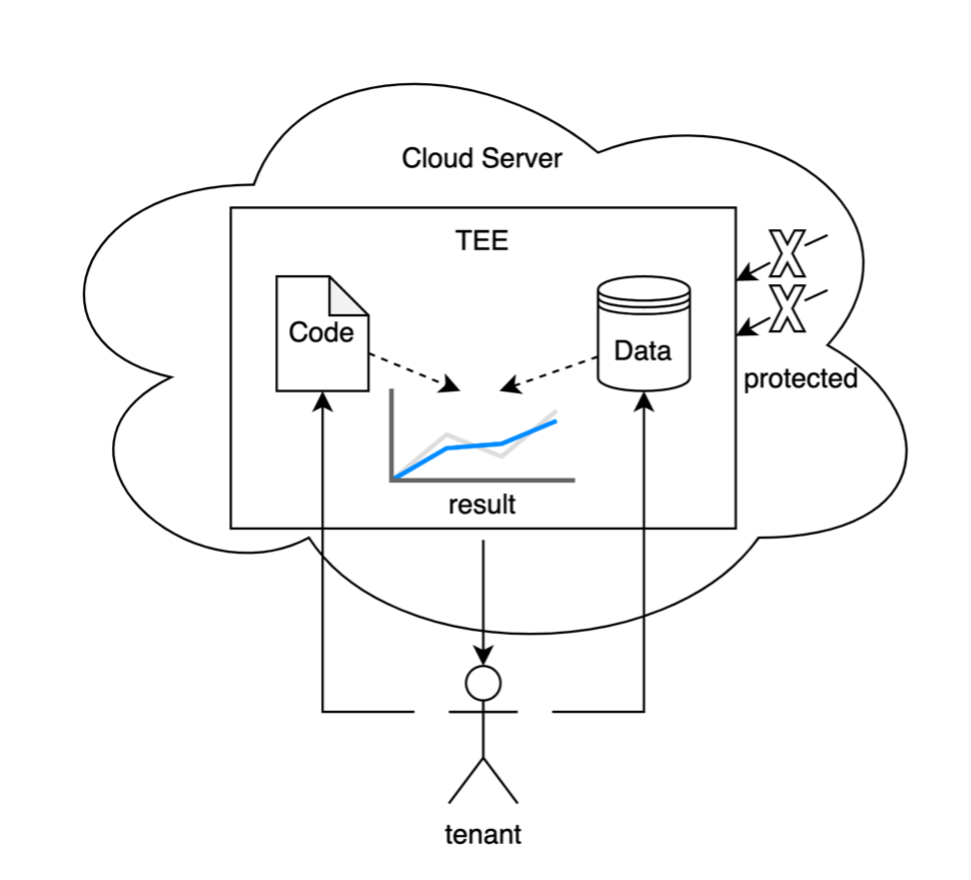
\includegraphics{images/analysis_2_roles.png}
        }
      } &
      \subfloat[multiple roles]{
  \hspace*{-1cm}
        \scalebox{0.42}{
        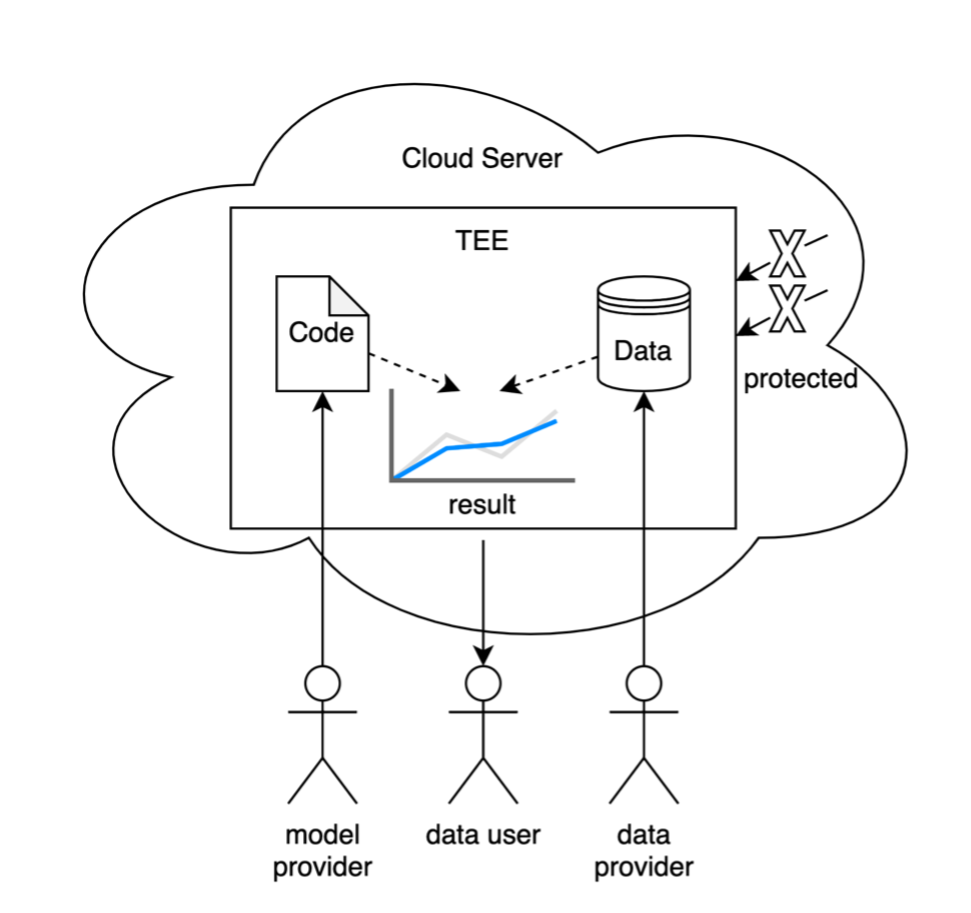
\includegraphics{images/analysis_4_roles.png}
        }
      }    \\
\end{tabular}
  }
  \caption{\small Data Analysis Scenarios with Two Roles vs. Multiple Roles.}
  \label{fig:analysis_scenarios}
\end{figure}
% 然而,这些相关的研究在解决复杂的数据分析场景时,仍存在一些限制。
However, these relevant studies still exhibit certain limitations when addressing these data analysis scenarios. 
% 首先,这些相关的研究工作不能保证数据分析结果中不会泄漏数据。虽然这些工作引入了数据使用规则,用以描述哪些人以什么样的价格访问哪些类型的数据,但对数据进行分析的程序是存在作恶的可能的,分析程序的最终输出结果可能是包含敏感信息泄漏的。一个最简单的例子是,分析程序直接输出原始数据,这样数据分析结果就获取到了完整的原始数据。
First, these related research efforts do not guarantee the prevention of data leakage within data analysis results. Although these works introduce data usage policies to describe who can access what kinds of data at what price, there is the possibility of malicious behavior in data analysis programs. The final output of the analysis program may include the leakage of sensitive information. An example is when the analysis program directly outputs the raw data, allowing the data analysis results to gain access to the complete, raw data.
% 一个straghtforward的解决方案是,要求分析程序公开,数据提供方可以审核分析程序是否存在泄漏数据的代码。但是对于模型提供方而言,模型也是他们重要的资产,他们不希望模型公开。另一方面,对于复杂的分析程序来说,审核分析程序存在巨大的工作量,不可能要求每一个分析任务都去进行审核,这会大大降低数据分析的效率。
A straightforward solution is to require the analysis program to be open and accessible for data providers to audit, ensuring that it does not contain code that could lead to data leaks. However, for model providers, their models are valuable assets, and they may be reluctant to make them publicly available. On the other hand, auditing complex analysis programs represents a significant workload, and it is not feasible to require audits for every analysis task, as this would significantly reduce the efficiency of data analysis.

% 结果可验证
% 其次,当前的工作中并不能保证计算结果的可信与可验证。具体来说,数据使用方得到计算结果后,他不能确定这个计算结果确实是通过指定的数据与指定的模型运行之后得到的计算结果,而不是一个随机生成的结果。更进一步,数据使用方并没有任何方式去验证这个结果的正确性。如果计算结果的可信和可验证都无法保证,那么完全可以用一个伪造的计算结果来欺骗数据使用方,数据使用方的利益将会受到损害。
Second, the existing works cannot ensure the trustworthiness and verifiability of computation results. Specifically, when a data user receives computation results, they are unable to confirm that these results indeed stem from running the specified data through the specified model and are not simply randomly generated. Furthermore, data users lack any means to validate the correctness of these results. Without the assurance of both trustworthiness and verifiability of the computation results, there is the potential for deceptive results to be used to mislead data users, jeopardizing their interests.

% 分析程序一致性
% 最后,当前的工作中每一次进行数据分析任务都需要使用remote attestation来保证分析程序的一致性,但是有相关工作表明,remote attestation具有低效、依赖可信第三方的缺点。
Finally, in existing works, remote attestation is required for every data analysis task to ensure the consistency of the analysis program. However, related works~\cite{chen2019opera,chen2022mage} have shown that remote attestation has drawbacks such as inefficiency and dependence on trusted third parties.
% 以Intel SGX中的Enhanced Privacy ID(EPID)为例,一次remote attestation的过程会涉及到Intel Provisioning Service(IPS)、Intel Attestation(IAS) Service、Intel-signed provisioning enclave(PvE)、Intel-signed quoting enclave(QE)以及分析程序Enclave之间的交互。这些服务和Enclaves之间的交互需要通过广域网传输数据,同时,传输的数据需要加密保证其安全性,对于频繁的数据分析任务而言,性能上会有较大的损失。另一方面,IPS和IAS是Intel提供的中心化服务,remote attestation需要依赖其稳定运行。
Taking Intel Software Guard Extensions (SGX) Enhanced Privacy ID (EPID) as an example, a single remote attestation process involves interactions between the Intel Provisioning Service (IPS), Intel Attestation Service (IAS), Intel-signed provisioning enclave (PvE), Intel-signed quoting enclave (QE), and the analysis program enclave. These interactions require data transmission over a wide area network, and the transmitted data must be encrypted to ensure its security. For frequent data analysis tasks, this can lead to significant performance overhead. On the other hand, IPS and IAS are centralized services provided by Intel, making remote attestation dependent on their stable working.

In this paper, we propose Fidelius, a system that leverages Intel SGX and blockchain to enhance data analysis security, addressing the previously mentioned limitations.
% 其中,Intel SGX保证数据分析过程的security和integrity,区块链用于可信的传输、存储和验证。
Intel SGX ensures the security and integrity of the data analysis process, while the blockchain is utilized for trustworthy transmission, storage, and verification.

% 为了解决计算结果泄漏数据的问题,Fidelius使用了静态二进制分析的方法,检查模型提供方的分析程序是否遵循隐私描述语言。其中,我们引入的隐私描述语言将数据的运算规则描述为有限状态机,反映了从输入数据到输出数据的状态转换,不在隐私描述语言描述的状态转换,都会被认为违反了隐私规则。
To address the issue of data leakage in computation results, Fidelius employs a static binary analysis approach~\cite{schulte2019gtirb} to examine whether the analysis program provided by the model adheres to a privacy description language (PDL). In this context, the introduced PDL characterizes the computational rules of data as a finite state machine (FSM), capturing the state transitions from input data to output data. Any state transitions not described in the PDL are considered as violations of the privacy rules.

% 为了解决计算结果的可信与可验证的问题,Fidelius提供了一套密码协议,该协议中由数据使用方提供一个私钥,该私钥通过加密转发至分析程序的Enclave中,并签名计算结果。由于该私钥仅在指定的分析程序Enclave中解密获得,数据提供方、模型提供方、云计算服务提供商均无法获取,故只要被签名的计算结果能够通过验证,说明计算结果确实出自指定的分析程序且可验证。
To ensure the trustworthiness and verifiability of computation results, Fidelius offers a cryptographic protocol. In this protocol, the data user provides a private key, which is securely transmitted to the analysis program's Enclave and used to sign the computation results. Since this private key can only be decrypted within the specified analysis program's Enclave, it remains inaccessible to the data provider, model provider, and cloud service provider. Therefore, if the signed computation results can be successfully verified, it confirms that the results indeed originate from the specified analysis program and are verifiable.

% 为了解决remote attestation低效、持续依赖中心化服务的问题,Fidelius结合设计的密码协议以及local attestation实现分析程序的一致性验证。Fidelius设计了密钥管理的Enclave,在初始化的过程中获取密钥的授权,在此后的所有数据分析任务中,使用该经授权的密钥执行local attestation完成分析程序的一致性验证。
To address the issues of the inefficiency and continued reliance on centralized services in remote attestation, Fidelius combines a designed cryptographic protocol with local attestation to achieve the consistency verification of analysis programs. Fidelius introduces a Key Management Enclave that obtains authorized keys during initialization. Subsequently, in all data analysis tasks, this authorized key is used to perform local attestation, ensuring the consistency of the analysis program.

The main contributions of this paper are summarized as follows.
\begin{itemize}
    \item First, we introduce the Privacy Description Language (PDL) combined with static binary analysis to rigorously enforce data confidentiality and prevent sensitive data leakage in computation outcomes.
    \item Second, we design a cryptographic protocol to ensure the trustworthiness and verifiability of computation results.
    \item we integrate the cryptographic protocol with a local attestation mechanism to ensure the integrity and correctness of analysis programs executed within protected environments.
    \item Finally, we evaluate the performance of Fidelius, and the experimental results demonstrate that it incurs minimal overhead, contributing less than 2\% to the data analysis system, while surpassing existing solutions by more than 30 times.
\end{itemize}




\section{Background}
\subsection{Intel SGX}
Intel Software Guard Extensions (SGX) is a hardware-level trusted execution environment that safeguards program execution. It establishes a secure, private memory region, called Enclave Page Cache (EPC), safeguarding its content from unauthorized access or modification by external processes. This designated memory space is considered trusted, while any region beyond it is deemed untrusted, strictly restricting access from untrusted environments.

A program deployed within the EPC is referred to as an enclave program. Enclaves are designed to operate in isolation from untrusted environments and can only interact through explicitly declared methods, known as ECALL or OCALL methods.

We will introduce the key methods and operations that are encapsulated within an enclave.
\begin{itemize}
\item $sgx\_get\_key()$: This function retrieves a symmetric key that is generated based on the hash of the current enclave, CPU ID, and other configuration files. Each enclave has a unique symmetric key generated in this manner. The symmetric key remains inaccessible from outside the enclave unless specific exporting (OCALL) methods are declared.
\item $sgx\_ecc256\_create\_key\_pair()$: This function generates an ECC-256 asymmetric key pair by utilizing SGX's self-contained random number generator.
\end{itemize}

To securely store private messages from an enclave in local storage, the "seal" operation employs the enclave's symmetric key to encrypt the message and then stores it locally. This approach ensures that the plaintext of the sealed message remains inaccessible to users, as the symmetric key remains undisclosed.
To unseal the message, users transmit the message to the enclave using a designated (ECALL) method, and the enclave decrypts the message using its own symmetric key.

\subsection{Remote Attestation}
% remote attestation是Intel提供的一种用于证明未知平台运行的enclave程序的integrity的技术。到目前为止,Intel支持的remote attestation的类型有两种:Intel Enhanced Privacy ID (Intel EPID) Attestation和Elliptic Curve Digital Signature Algorithm (ECDSA) Attestation。
Remote attestation is a technology provided by Intel SGX to prove the integrity of enclave programs running on an unknown platform. Currently, Intel SGX provides two types of remote attestation: Intel Enhanced Privacy ID (Intel EPID) Attestation and Elliptic Curve Digital Signature Algorithm (ECDSA) Attestation.

% 基于EPID的remote attestation一般包括如下步骤。首先,应用程序enclave向同平台的quoting enclave发起请求,生成应用程序enclave的quote。其中,quoting enclave是Intel SGX官方提供的enclave。这两个enclave之间通过local attestation进行请求发送、quote传输,其中,local attestation仅为同一平台的两个enclave之间建立可信通道并进行数据传输。应用程序enclave在接收到quote之后,向远端的Intel Attestation Service发送,进行验证,得到验证的结果。
Remote attestation based on EPID typically involves the following steps. The application enclave initiates a request to the local quoting enclave (QE) provided by Intel SGX, generating a quote for the application enclave. These two enclaves use local attestation for request initiation and quote transmission, wherein local attestation establishes a trusted channel and enables data transfer between two enclaves on the same platform. After receiving the quote, the application enclave sends it to the remote Intel Attestation Service (IAS) for verification and obtains the verification result.
% EPID存在着诸多限制,例如,要求应用程序enclave所在的网络能够连接上Intel Attestation Service,要求Intel Attestation Service服务在任何时候都高可用(即不存在单点故障或者下线)。
EPID has several limitations, such as requiring that the network where the application enclave is located can connect to the Intel Attestation Service. It also demands that the Intel Attestation Service is highly available at all times, meaning there are no single points of failure or downtime.

ECDSA-based Attestation was introduced to address the limitations associated with EPID. With Intel SGX Data Center Attestation Primitives (DCAP), ECDSA-based attestation enables providers to establish and offer a third-party attestation service, eliminating the need to rely on Intel's provided remote attestation service.
% Intel SGX DCAP允许第三方提供quoting enclave,并生成应用程序enclave的quote。其中,第三方quoting enclave使用的attestation key可由data center内部生成。attestation key的公钥将被发送至Intel's Provisioning Certification Enclave (PCE)并被签名/授权。在生成quote之后,quote会发送给data center内部的attestation service进行验证。
Intel SGX DCAP allows third parties to provide a quoting enclave and generate quotes for application enclaves. The attestation key used by the third-party quoting enclave can be generated internally within the data center. The public key of the attestation key is sent to Intel's Provisioning Certification Enclave (PCE) and signed/authorized. After generating the quote, it is sent to the data center's internal attestation service for verification.

% SGX offers two types of communication between enclaves: local attestation (LA) and remote attestation (RA). Local attestation is limited to two enclaves on the same platform, while remote attestation facilitates cross-platform communication. During local attestation, each enclave can validate the hash value or the signer of the interacting enclave. In contrast, remote attestation requires a trusted third party, such as an Intel server or DCAP, to verify this information.

\subsection{Blockchain}
\subsubsection{Permissionless Chain and Permissioned Chain}
% 区块链分为公链和联盟链,公链所有人都可以访问,一个节点可以任意加入或者离开,没有任何权限控制。由于公链限制少,达成所有节点的共识就相对困难,导致其系统吞吐较低。公链最开始用于跨境支付,后发展成为去中心化金融的底层技术框架。联盟链顾名思义,由多个联盟成员组成,联盟成员一般为企业、机构、政府单位等。联盟链作为联盟成员中的可信第三方,具备公开、透明的特点,主要用于数据的公开存证、溯源、验证等。由于联盟链中的成员数量不多,可通过高效的共识算法使其达成一致,因此联盟链具备较高的吞吐性能。
Blockchain can be categorized into permissionless chains and permissioned chains. In permissionless chains, accessibility is open to everyone, and nodes can freely join or leave without any permission control. Due to the limited restrictions in permissionless chains, achieving consensus among all nodes can be relatively challenging, resulting in lower system throughput. Permissionless chains initially found application in cross-border payments and later evolved into the foundational technology framework for decentralized finance.

Permissioned chains consist of multiple members, which are typically comprised of enterprises, institutions, government entities, and similar organizations. Permissioned chains serve as trusted third parties, offering characteristics of openness and transparency. They are primarily used for public data notarization, traceability, verification. Due to the smaller number of members in permissioned chains, efficient consensus algorithms can be employed to facilitate consensus among them, thereby endowing permissioned chains with higher throughput performance.

In Fidelius, the utilization of permissioned blockchain serves as a reliable and fault-tolerant third-party entity for tasks like data transmission, data storage. In contrast, traditional mediators are susceptible to single point failures, data tampering risks, and the high costs associated with establishing P2P private networks.

\subsubsection{Smart Contract}
Blockchain's smart contracts are on-chain programs known for their transparency in code and execution processes. In Fidelius, smart contracts play a pivotal role in verifying the signature of the analysis results provided by cloud service providers. The success of a data analysis is assured once the verification is successfully completed, instilling trust in all parties involved.

%\subsection{Binary Analysis}


\section{Threat Model and Design Choice}

In this section, we first introduce the roles within the system, then detail the threat model, highlighting potential risks and discussing various types of attacks. Additionally, we establish key assumptions that form the foundation for the design and implementation of Fidelius. Subsequently, we delve into the design choices made for Fidelius, aimed at mitigating the identified risks and countering potential attacks on the system.

\subsection{Roles}
\begin{itemize}
    \item Data Provider (DP). Data provider, as the sole owner of the raw data, initially publishes metadata on the blockchain, which includes the hash and a necessary description of the raw data. The accuracy of this metadata is validated by the data provider's credibility, exemplified by a history of successful data analyses.
    \item Model Provider (MP). Model provider supplies analysis programs for specific types of data.
    \item Cloud Service Provider (CSP). Cloud computing provider supplies the computational resources required for data analysis and additionally provides a Trusted Execution Environment to ensure secure data analysis. After receiving a request for a data analysis task, the cloud computing provider is obligated to execute the analysis program and return the results to the blockchain.
    \item Data User (DU). Data user selects the desired raw data by examining the metadata on the blockchain and initiates a data analysis to obtain the results from the specified analysis program.
    \item Blockchain. Blockchain serves as a reliable, failure-resistant third party for data transmission and storage. Specifically, a smart contract verifies the correctness of the signature on the analysis results.
\end{itemize}

\subsection{Threat Model}\label{subsec:threatmodel}
% 系统包含数据提供方、模型提供方、云服务提供方以及数据适用方四个角色,四个角色之间是相互不信任的。

The system comprises four distinct roles: data provider, model provider, cloud service provider, and data user, which are inherently distrustful of one another.
% 在数据分析的过程中,存在以下攻击:
% 数据窃取攻击:模型提供方的模型逻辑存在窃取原始数据或者中间数据的恶意代码;云服务提供方通过提供的硬件或软件资源窃取数据;数据使用方登录进服务器窃取数据。
% 数据伪造攻击:数据提供方提供的数据和声称的不一致。
% 数据滥用攻击:数据提供方的数据被使用在不同的模型、不同的云服务器上。
% 结果伪造攻击:数据分析的结果并不是模型如实运行得到的。
% 结果窃取攻击:数据分析的结果被数据提供方、模型提供方、云服务提供方或未知的攻击者获取。
During the data analysis process, the following attacks are prevalent:
\begin{itemize}
    \item Data Theft Attacks: Cloud service provider may steal data through the hardware or software resources they provide; data user may log into the server to steal data. The program provided by the model provider may contain malicious code aimed at stealing raw or intermediate data.
    \item Data Fabrication Attacks: The data provided by the data provider is inconsistent with what is claimed.
    \item Data Misuse Attacks: Data from the data provider is used across different models and cloud servers without proper authorization.
    \item Result Fabrication Attacks: The results of the data analysis do not accurately reflect the true execution of the model.
    \item Result Theft Attacks: The results of data analysis are illicitly accessed by the data provider, model provider, cloud service provider, or an unidentified attacker.
\end{itemize}

We do not address side-channel attacks on Intel SGX in this paper. We assume Intel SGX's hardware functionality is as advertised, ensuring that code within an enclave remains unaltered and the values of internal variables are protected from direct memory access. Notably, our reliance on Intel is limited to a one-time interaction during the setup process; no further contact with Intel servers or DCAP is necessary. In contrast, previous approaches rely on remote attestation, requiring ongoing integrity and availability of Intel servers or DCAP for each data analysis task.

We assume the presence of a collision-resistant hash function and secure signature and encryption schemes. Specifically, our signatures incorporate a \textit{nonce} to ensure that a valid signature pair $(msg, signed_{msg})$ cannot be generated by an adversary without the private key, rendering historical signatures invalid.


\subsection{Design Choice}\label{subsec:designchoice}
To counter the identified attacks, we have made the following design choices.
% 抵御数据窃取攻击:所有存在于非可信环境(例如网络传输、云服务器的非TEE部分)的数据都经过加密处理,以防止数据使用方或云服务提供商直接窃取数据。模型提供方提供的分析程序,在进行数据分析前进行代码静态分析,防止模型提供方通过数据分析结果窃取数据。
% 抵御数据伪造攻击:执行数据分析前,检查数据哈希与声称的哈希是否一致。
% 抵御数据滥用攻击:引入数字签名技术,数据提供方用私钥签名使用数据的平台、模型以及模型的参数,在执行数据分析前,会验证该签名的有效性。
% 抵御结果伪造攻击:将数据使用方的私钥加密地传输到云服务器的可信执行环境中,并用这个私钥签名结果。当数据使用方拿到结果时,也会得到该私钥对结果的签名,若签名验证通过,说明结果确实是由可信执行环境中得到的,故结果未经伪造。这一思想类似于零知识证明。
% 抵御结果窃取攻击:数据分析结果由数据使用方的公钥加密,只能被数据使用方查看。
\begin{itemize}
    \item Defending Against Data Theft Attacks: All data located in non-trusted environments, such as network transmissions or the non-TEE components of cloud servers, are encrypted to prevent direct data theft by data users or cloud service providers. Additionally, the analysis programs provided by model providers undergo static code analysis prior to data analysis to prevent data theft through the analysis results.
    \item Defending Against Data Fabrication Attacks: Prior to conducting data analysis, the data hashes are verified to ensure they match the claimed hashes.
    \item Defending Against Data Misuse Attacks: Digital signature technology is implemented, enabling the data provider to sign the platform, model, and model parameters using a private key. The validity of this signature is verified before executing data analysis.
    \item Defending Against Result Fabrication Attacks: The data user's private key is securely transmitted to the Trusted Execution Environment (TEE) on the cloud server and used to sign the results. When the data user receives the results, they also receive the signature made by the private key. If the signature is validated, it confirms that the results were indeed obtained from the TEE, ensuring the results have not been fabricated. This approach is analogous to zero-knowledge proof.
    \item Defending Against Result Theft Attacks: The results of data analysis are encrypted with the data user's public key, ensuring that only the data user can access them.
\end{itemize}

\section{Design}\label{sec:design}

\subsection{Overview}
This section provides a brief overview of the enclaves and notations used in Fidelius, along with its architecture and workflow.

% 英文版原始内容(如无legend相关内容则无需更改)

\subsubsection{Enclaves and Notations}
Throughout this paper, we define the following enclaves and notations:
\begin{itemize}
    \item EKeyMgr. Enclave Key Manager manages asymmetric keys, handling creation, deletion and provides fundamental cryptographic functions, including message encryption, decryption, signing, and signature verification.
    \item EAnalyzer. Enclave Analyzer, an analysis program in Intel SGX Enclave format, ensures the program remains unaltered during execution.
    \item $(PK_{DP},SK_{DP})$, an asymmetric key pair of data provider.
    \item $(PK_{DU},SK_{DU})$, an asymmetric key pair of data user.
    \item $(PK_{CSP}, SK_{CSP})$ represents the asymmetric key pair of cloud service provider, generated by EKeyMgr. The private key, $SK_{CSP}$, is securely stored within the enclave, ensuring that it cannot be extracted by the cloud service provider.
    \item $H(\cdot)$ denotes the hash function.
    \item $Enc(PK, msg)$ denotes the encryption of $msg$ using $PK$.
    \item $Dec(SK, cipher)$ denotes the decryption of $cipher$ using $SK$.
    \item $Sign(SK, msg)$ denotes the signing of $msg$ with $SK$.
    \item $Verf(PK, msg, sig)$ denotes the verification of $sig$ using $PK$ and $msg$.
    \item $\digamma(SK, PK_{CSP}, H_{EA})$ represents the process of forwarding $SK$ to EKeyMgr using $PK_{CSP}$. Within this context, $SK$ is utilized in EAnalyzer, identified by $H_{EA}$. The function $\digamma(\cdot)$ involves $Sign(SK, concat(PK_{CSP}, H_{EA}))$ and $Enc(PK_{CSP}, SK)$.
\end{itemize}

\subsubsection{Architecture and Workflow}

The Fidelius architecture and data analysis workflow are illustrated in Figure~\ref{fig:arch}. 
The process begins with a setup phase where the EKeyMgr in CSP generates an asymmetric key pair. The public key, $PK_{CSP}$, undergoes verification via Intel's remote attestation service, while the private key, $SK_{CSP}$, remains securely stored within EKeyMgr. Concurrently, the Data Provider (DP) and Data User (DU) each generate their own asymmetric key pairs, which they retain. Additionally, the DP encrypts data using her public key, $PK_{DP}$, and prepares this encrypted data for the DU's use.

The DP uploads encrypted data to the CSP and forwards her private key, $SK_{DP}$, to EKeyMgr using $\digamma(SK_{DP}, PK_{CSP}, H_{EA})$. Similarly, the DU uploads the analysis program to the CSP and forwards her private key, $SK_{DU}$, to EKeyMgr using the same method. It is important to note that the plaintext private keys ($SK_{DP}$ and $SK_{DU}$) can only be decrypted within EKeyMgr.

Once the analysis program, encrypted data, and private key are prepared, the data analysis task begins. The analysis program is first checked against the rules defined by the Privacy Description Language (PDL). Any program that fails this check results in an immediate termination of the analysis task. Subsequently, EAnalyzer loads and decrypts the encrypted data. It then verifies the hash of the decrypted data; if it does not match the claimed hash, EAnalyzer halts immediately to prevent processing altered or fraudulent data. If the data is verified, EAnalyzer proceeds with the main analysis, ultimately producing an encrypted result using $PK_{DU}$. Additionally, the result is signed using $SK_{DU}$. Since $SK_{DU}$ resides within EKeyMgr, EAnalyzer establishes a secure channel via local attestation to request $SK_{DU}$.

% 英文版原始内容(如无legend相关内容则无需更改)

\subsection{Privacy Description Language}
% 为了防止数据分析结果泄漏数据,我们提出了隐私描述语言来定义使用数据的规则,并通过了静态⼆进制分析的⽅法检查分析程序是否遵守隐私描述语言定义的规则。如图所示,这段代码使用PDL描述了在Iris数据集上使用Kmeans算法的规则,这段代码也将被转换成LLVM的中间表示,然后使用符号执行得到PDL描述的规则的状态a。另一方面,我们使用GTIRB作为分析的中间表⽰,在将分析程序转换为中间表⽰后,使⽤符号执⾏获取每个输出变量的状态b,并判断是否满足b包含于a。
To prevent data leakage from analysis results, we have developed a Privacy Description Language (PDL) that defines rules for data usage. Static binary analysis is used to ensure that the analysis program adheres to these PDL-defined rules. As illustrated in Figure~\ref{fig:pdl}, the code snippet uses PDL to specify the rules for applying the KMeans algorithm on the Iris dataset. This code is then translated into LLVM's intermediate representation (IR), followed by symbolic execution~\cite{king1976symbolic,baldoni2018survey} to derive the state $S$ as described by PDL. Concurrently, we utilize GTIRB~\cite{schulte2019gtirb} for intermediate representation in our analysis. After converting the analysis program to this format, symbolic execution is applied to obtain the state $S^{\prime}$ of each output variable, ensuring that $S^{\prime}$ is a subset of $S$, thereby confirming compliance.

\subsection{Trustworthy and Verifiable Results}
Algorithm~\ref{algo:analysis_enclave} outlines the primary operations of EKeyMgr and EAnalyzer. The encrypted analysis result and its signature, generated within EAnalyzer, are transmitted to the blockchain. There, anyone can verify the signature's validity. A valid signature confirms that the DP successfully executed the analysis program and achieved the correct result, since the signature originates from within EAnalyzer. This mechanism prevents attackers from forging a valid signature without executing the analysis program, thereby ensuring the integrity of the data analysis process. The DU can download the encrypted result from the blockchain and decrypt it using $SK_{DU}$ to obtain the plaintext analysis result.
% 英文版原始算法内容(如无legend相关内容则无需更改)


\subsection{One-time Remote Attestation}
%We implement a one-time remote attestation as outlined in Algorithm~\ref{algo:attestation}. 
We incorporate a one-time remote attestation process, as detailed in Algorithm \ref{algo:attestation}, to establish a secure and trusted environment from the outset. 
%During the setup phase, the Cloud Service Provider (CSP) verifies the authorization of $PK_{CSP}$, generated by EKeyMgr, through a remote attestation with Intel service. 
During the setup phase, the Cloud Service Provider (CSP) validates the authorization of the public key $PK_{CSP}$ generated by EKeyMgr by performing a remote attestation with Intel’s attestation service. This thorough verification confirms both the integrity and legitimacy of the CSP’s credentials.
Once verified, subsequent analysis tasks on the CSP no longer require remote attestation. The private keys ($SK$) forwarded by the DP and DU are securely transmitted from EKeyMgr to EAnalyzer via local attestation.
%We incorporate a one-time remote attestation process, as detailed in Algorithm \ref{algo:attestation}, to establish a secure and trusted environment from the outset. During the initial setup phase, the Cloud Service Provider (CSP) rigorously validates the authorization of the public key $PK_{CSP}$ generated by EKeyMgr by performing a remote attestation with Intel’s attestation service. This thorough verification confirms both the integrity and legitimacy of the CSP’s credentials. Once this attestation is successfully completed, all subsequent analysis tasks on the CSP can be executed without further attestation, thereby streamlining operations and reducing overhead. Additionally, the private keys ($SK$) supplied by the DP and DU are securely transmitted from EKeyMgr to EAnalyzer via a robust local attestation process, ensuring that sensitive cryptographic material remains confidential and tamper-resistant throughout the transfer.

\section{Evaluation}\label{sec:eval}
% 英文版原始算法内容(如无legend相关内容则无需更改)

In this section, we assess Fidelius's performance through comprehensive experiments. Initially, we gauge its time consumption by executing CPU-intensive and I/O-intensive tasks separately. Subsequently, we conduct a performance comparison between Fidelius and alternative solutions that execute analysis programs in the Ethereum Virtual Machine (EVM). Our experiments are conducted on a machine equipped with an Intel(R) Core(TM) i5-10400F CPU boasting 12 cores at 2.9 GHz, 16 GBytes of RAM, and a 12 MByte cache. Unless otherwise stated, each experiment is repeated 1,000 times to calculate the average value.

\subsection{CPU-Intensive Task}
To evaluate Fidelius's performance on CPU-intensive tasks, we implement a neural network algorithm with three layers and 128 hidden units, designed to recognize handwritten digits using the MNIST dataset~\cite{mnist}. We report both the time consumption and accuracy of the algorithm. Additionally, we deploy the algorithm on raw CPU (without SGX) for comparison. The key differences between the Fidelius-based algorithm and the raw CPU-based algorithm include:
\begin{itemize}
  \item Random library. The Fidelius-based algorithm utilizes a random library based on Intel SGX, whereas the raw CPU-based algorithm relies on the C++ random library.
  \item Data decryption. Fidelius requires decryption of sealed data before initiating the algorithm, incurring additional processing time. Conversely, the raw CPU-based algorithm can directly access plaintext data.
\end{itemize}
Both for Fidelius and raw CPU, we maintain a fixed number of test sets at 1,000 while incrementally increasing the number of training sets from 10,000 to 50,000. For each training set, we execute the algorithm with epochs set to 100 and 200, respectively.


\begin{figure*}[h]
\centering
{
  \setlength{\tabcolsep}{0pt}
  \begin{tabular}{cccc}
\subfloat[epoch = 100]{
  \scalebox{0.39}{
  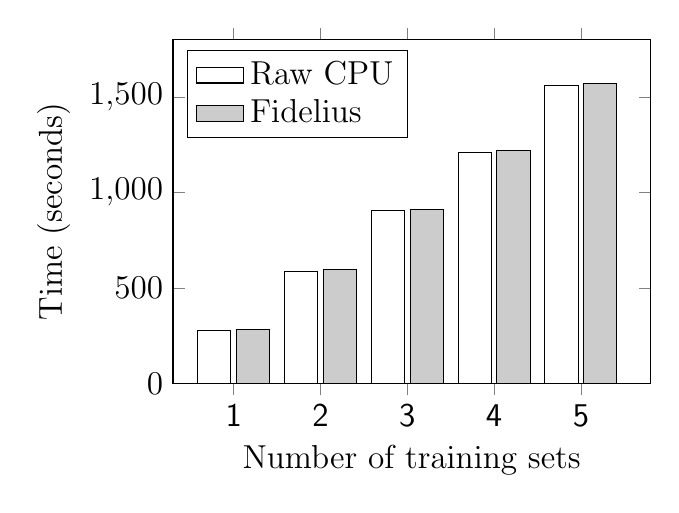
\begin{tikzpicture}
    
\begin{axis}[
  compat=newest,
  legend style={
     legend columns=1,
     font=\large,
     legend pos=north west},
  ybar,
  bar width=12pt,
  ymin=0,
  ymax=1800,
  xmin=0.3,
  xmax=5.8,
  scale only axis,
  xticklabels={\bench{\large 1}, \bench{\large 2}, \bench{\large 3},
    \bench{\large 4}, \bench{\large 5}
  },
  ylabel={Time (seconds)
  },
    xlabel=Number of training sets,
    xtick=data,
    width=0.5\textwidth,
    height=0.36\textwidth,
    every axis/.append style={font=\large,
      label style={font=\large},
      tick label style={font=\large}
    }
  ]
\addplot [area legend] coordinates{
  (1, 278.258)
  (2, 587.359)
  (3, 905.65)
  (4, 1208.9)
  (5, 1562.5)
};
\addplot [fill=black!20,area legend] coordinates{
  (1, 282)
  (2, 595.27)
  (3, 909.03)
  (4, 1219.71)
  (5, 1570)
};
\legend{[right]{Raw CPU}, [right]{Fidelius}}
\end{axis}
\end{tikzpicture}}
} &
\subfloat[epoch = 200]{
  \scalebox{0.39}{
  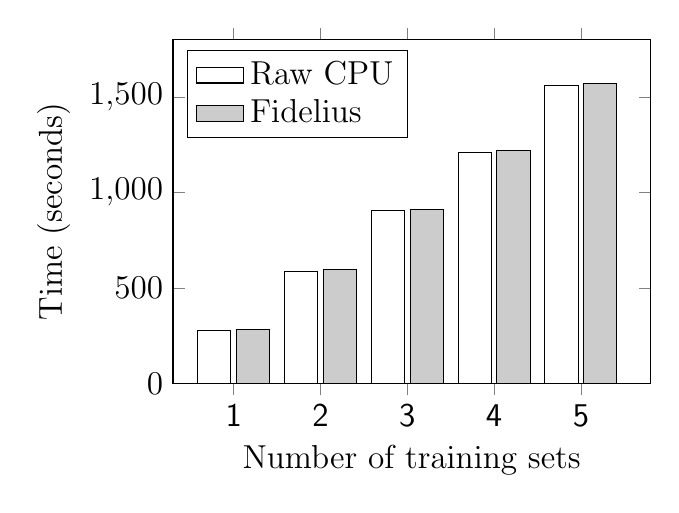
\begin{tikzpicture}
    
\begin{axis}[
  compat=newest,
  legend style={
     legend columns=1,
     font=\large,
     legend pos=north west},
  ybar,
  bar width=12pt,
  ymin=0,
  ymax=1800,
  xmin=0.3,
  xmax=5.8,
  scale only axis,
  xticklabels={\bench{\large 1}, \bench{\large 2}, \bench{\large 3},
    \bench{\large 4}, \bench{\large 5}
  },
  ylabel={Time (seconds)
  },
    xlabel=Number of training sets,
    xtick=data,
    width=0.5\textwidth,
    height=0.36\textwidth,
    every axis/.append style={font=\large,
      label style={font=\large},
      tick label style={font=\large}
    }
  ]
\addplot [area legend] coordinates{
  (1, 278.258)
  (2, 587.359)
  (3, 905.65)
  (4, 1208.9)
  (5, 1562.5)
};
\addplot [fill=black!20,area legend] coordinates{
  (1, 282)
  (2, 595.27)
  (3, 909.03)
  (4, 1219.71)
  (5, 1570)
};
\legend{[right]{Raw CPU}, [right]{Fidelius}}
\end{axis}		
\end{tikzpicture}}
} &
\subfloat[epoch = 100]{
  \scalebox{0.39}{
  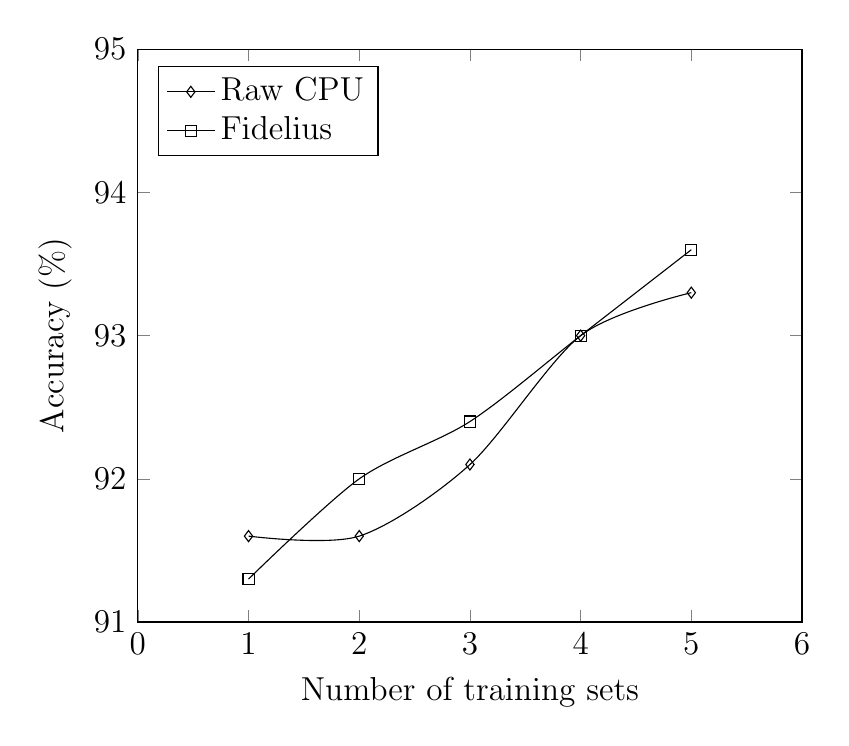
\begin{tikzpicture}
    
\large
\pgfplotsset{
    scale only axis,
    xmin=0, xmax=6,
    compat=newest,
    legend pos=north west,
}

\begin{axis}[
  %axis y line*=left,
  %scaled y ticks=base 10:2,
  %ymin=0, ymax=0.0004,
  %ymin=0, ymax=0.008,
  ymin=91, ymax=95,
  xlabel=Number of training sets,
  %width=0.4\textwidth,
  %height=0.6\textwidth,
  ylabel=Accuracy (\%),
]

\addplot[smooth,mark=diamond]
  coordinates{
    (1,91.6)
    (2,91.6)
    (3,92.1)
    (4,93.0)
    (5,93.3)
}; \label{plot_raw}

\addplot[smooth,mark=square]
  coordinates{
    (1,91.3)
    (2,92.0)
    (3,92.4)
    (4,93.0)
    (5,93.6)
  }; \label{plot_fid}



  \addlegendimage{/pgfplots/refstyle=plot_raw}\addlegendentry[right]{Raw CPU}
  \addlegendimage{/pgfplots/refstyle=plot_fid}\addlegendentry[right]{Fidelius}

\end{axis}
\end{tikzpicture}}
} &
\subfloat[epoch = 200]{
  \scalebox{0.39}{
  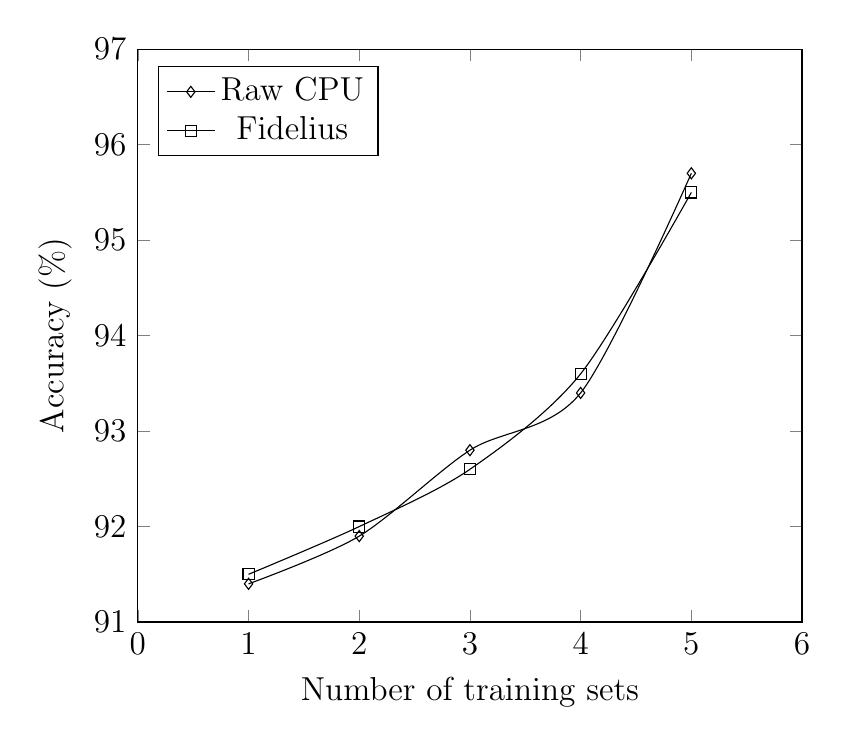
\begin{tikzpicture}
    
\large
\pgfplotsset{
    scale only axis,
    xmin=0, xmax=6,
    compat=newest,
    legend pos=north west,
}

\begin{axis}[
  %axis y line*=left,
  %scaled y ticks=base 10:2,
  %ymin=0, ymax=0.0004,
  %ymin=0, ymax=0.008,
  ymin=91, ymax=97,
  xlabel=Number of training sets,
  %width=0.4\textwidth,
  %height=0.6\textwidth,
  ylabel=Accuracy (\%),
]

\addplot[smooth,mark=diamond]
  coordinates{
    (1,91.4)
    (2,91.9)
    (3,92.8)
    (4,93.4)
    (5,95.7)
}; \addlegendentry{Raw CPU}

\addplot[smooth,mark=square]
  coordinates{
    (1,91.5)
    (2,92.0)
    (3,92.6)
    (4,93.6)
    (5,95.5)
  }; \addlegendentry{Fidelius}

\end{axis}
\end{tikzpicture}}
} \\
\end{tabular}
}
  \caption{\small Time Consumption and Accuracy of CPU-Intensive Task.}
\label{fig:cpu_intensive}
\end{figure*}


Figures~\ref{fig:cpu_intensive}(a) and~\ref{fig:cpu_intensive}(b) illustrate the time consumption of the algorithms running on Fidelius and raw CPU with varying epochs. As the number of training sets increases, the time consumption of the algorithms on both Fidelius and raw CPU shows a linear growth trend. However, the time consumption difference between these two algorithms is minimal. Specifically, it is observed that the execution time on Fidelius is only 2\% longer than that of raw CPU, primarily due to data decryption overhead.

Figures~\ref{fig:cpu_intensive}(c) and~\ref{fig:cpu_intensive}(d) show the accuracy of algorithms on Fidelius and raw CPU over different epochs, with both achieving over 91\% accuracy. At 100 epochs, accuracy fluctuates slightly, but with no marked difference between the platforms. At 200 epochs, both algorithms converge with nearly identical accuracies. Fidelius shows a marginal 2\% increase in time consumption compared to raw CPU but maintains similar accuracy levels, demonstrating comparable performance in CPU-intensive tasks.


\subsection{I/O-Intensive Task}\label{subsec:io_intensive}
To evaluate the time efficiency of Fidelius in handling I/O-intensive tasks, we tested an algorithm that searches for a target string within a file over 1 GByte on both Fidelius and raw CPU platforms. Time consumption depends on data loading and string searching, with additional time required on Fidelius due to data decryption. Given Intel SGX's constraints in Fidelius, we set data loading block sizes to 64 KBytes and 256 KBytes and varied the number of data lines from 1 to 128 and 1 to 256 for each block size to measure time efficiency.



\begin{figure}[h]
  \centering
{
\begin{tabular}{cc}
      \subfloat[Data block size = 64 KBytes]{
        \scalebox{0.39}{
          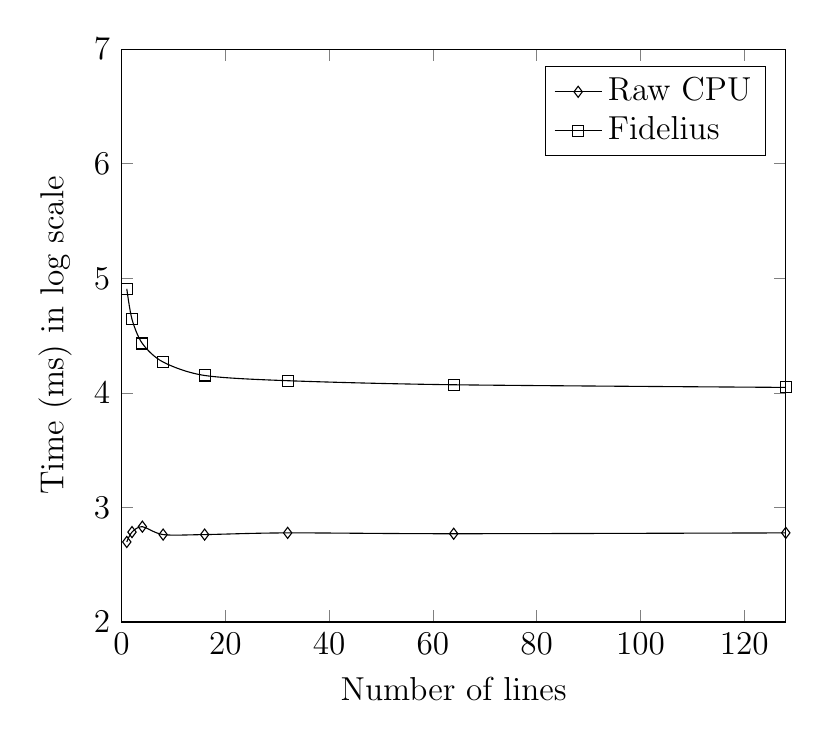
\begin{tikzpicture}
            
\large
\pgfplotsset{
    scale only axis,
    xmin=0, xmax=128,
    compat=newest,
    legend pos=north east,
}

\begin{axis}[
  %axis y line*=left,
  %scaled y ticks=base 10:2,
  %ymin=0, ymax=0.0004,
  %ymin=0, ymax=0.008,
  ymin=2, ymax=7,
  xlabel=Number of lines,
  %width=0.4\textwidth,
  %height=0.6\textwidth,
  ylabel=Time (ms) in log scale,
]

\addplot[smooth,mark=diamond]
  coordinates{
    (1,2.6990) %log10(500)
    (2,2.7853) %log10(610)
    (4,2.8325) %log10(680)
    (8,2.7634) %log10(580)
    (16,2.7634) %log10(580)
    (32,2.7782) %log10(600)
    (64,2.7709) %log10(590)
    (128,2.7782) %log10(600)
}; \label{plot_raw}

\addplot[smooth,mark=square]
  coordinates{
    (1,4.9085) %log10(81000)
    (2,4.6435) %log10(44000)
    (4,4.4314) %log10(27000)
    (8,4.2695) %log10(18600)
    (16,4.1523) %log10(14200)
    (32,4.1065) %log10(12780)
    (64,4.0711) %log10(11780)
    (128,4.0481) %log10(11170)
  }; \label{plot_fid}



  \addlegendimage{/pgfplots/refstyle=plot_raw}\addlegendentry[right]{Raw CPU}
  \addlegendimage{/pgfplots/refstyle=plot_fid}\addlegendentry[right]{Fidelius}

\end{axis}
          \end{tikzpicture}
        }
      } &
      \subfloat[Data block size = 256 KBytes]{
        \scalebox{0.39}{
          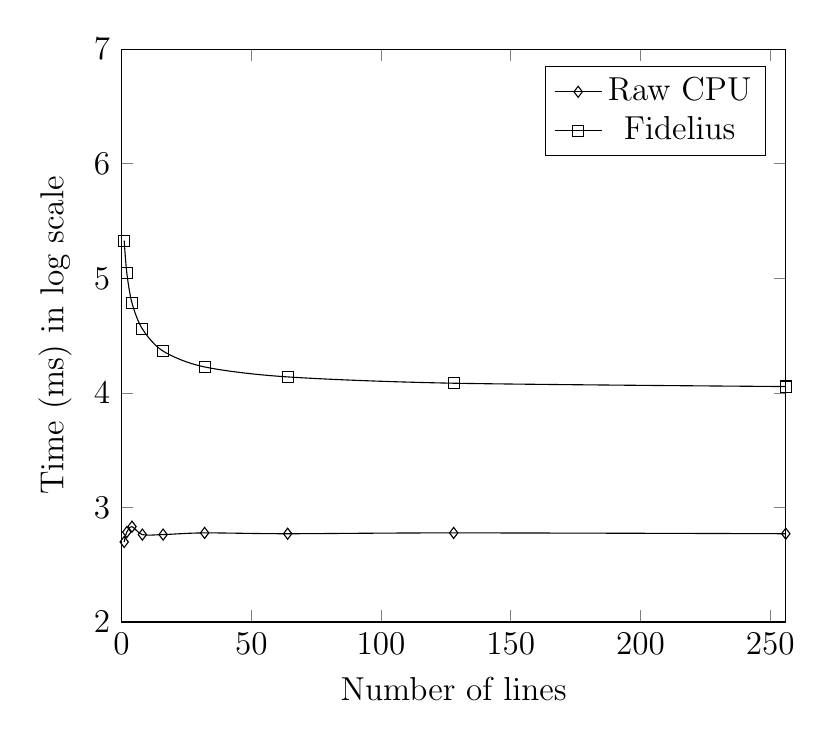
\begin{tikzpicture}
            
\large
\pgfplotsset{
    scale only axis,
    xmin=0, xmax=256,
    compat=newest,
    legend pos=north east,
}

\begin{axis}[
  %axis y line*=left,
  %scaled y ticks=base 10:2,
  %ymin=0, ymax=0.0004,
  %ymin=0, ymax=0.008,
  ymin=2, ymax=7,
  xlabel=Number of lines,
  %width=0.4\textwidth,
  %height=0.6\textwidth,
  ylabel=Time (ms) in log scale,
]
1	0.5	    213
2	0.61	111.78
4	0.68	61.04
8	0.58	36.2
16	0.58	23.16
32	0.6	    16.85
64	0.59	13.79
128	0.6	    12.15
256	0.59	11.36
\addplot[smooth,mark=diamond]
  coordinates{
    (1,2.6990) %log10(500)
    (2,2.7853) %log10(610)
    (4,2.8325) %log10(680)
    (8,2.7634) %log10(580)
    (16,2.7634) %log10(580)
    (32,2.7782) %log10(600)
    (64,2.7709) %log10(590)
    (128,2.7782) %log10(600)
    (256, 2.7709) %log10(590)
}; \addlegendentry{Raw CPU}

\addplot[smooth,mark=square]
  coordinates{
    (1,5.3284) %log10(213000)
    (2,5.0484) %log10(111780)
    (4,4.7856) %log10(61040)
    (8,4.5587) %log10(36200)
    (16,4.3647) %log10(23160)
    (32,4.2266) %log10(16850)
    (64,4.1396) %log10(13790)
    (128,4.0846) %log10(12150)
    (256,4.0554) %log10(11360)
  }; \addlegendentry{Fidelius}

\end{axis}
          \end{tikzpicture}
        }
      }    \\
\end{tabular}
  }
  \caption{\small Time Consumption of I/O-Intensive Task.}
  \label{fig:io_intensive}
\end{figure}

Figure~\ref{fig:io_intensive} shows the time efficiency of Fidelius compared to raw CPU across different data block sizes. Fidelius shows a significant reduction in time consumption as the number of lines read increases. For instance, with a block size of 64 KBytes, the time taken by Fidelius drops from 81 seconds (for 1 line) to 11 seconds (for 128 lines). Similarly, with a block size of 256 KBytes, it reduces from 213 seconds (for 1 line) to 10 seconds (for 256 lines). Increasing the block size to 256 KBytes further optimizes Fidelius's performance. Despite improvements, a gap remains in time consumption between Fidelius and raw CPU, largely due to the decryption process in I/O-intensive tasks.

\subsection{Performance Comparison}\label{subsec:evm_cmp}
In this section, we compare the performance of Fidelius with SDTE~\cite{dai2019sdte}, which uses a \textit{k}-nearest neighbors (\textit{k}-NN) algorithm as an Ethereum smart contract to execute machine learning tasks on the Ethereum Virtual Machine (EVM). We implement the \textit{k}-NN algorithm on both Fidelius and raw CPU to evaluate each solution's time consumption, using the Titanic~\cite{titanic} dataset from Kaggle as input.

To evaluate the \textit{k}-NN algorithm's execution time on the Ethereum Virtual Machine (EVM), we deployed the \textit{k}-NN smart contract on Ganache, a personal Ethereum blockchain. The reported time consumption for \textit{k}-NN on the EVM focuses solely on the execution time, excluding any time spent on transaction broadcasting or committing. We also exclude the time required to upload the Titanic dataset to the blockchain, as the \textit{k}-NN contract uses on-chain data. Due to EVM's memory limits, the \textit{k}-NN algorithm cannot handle more than 60 test sets, hence we limit test sets to 10-60 while keeping training sets at 100.


\begin{figure}[h]
\centering
\scalebox{.8}
{
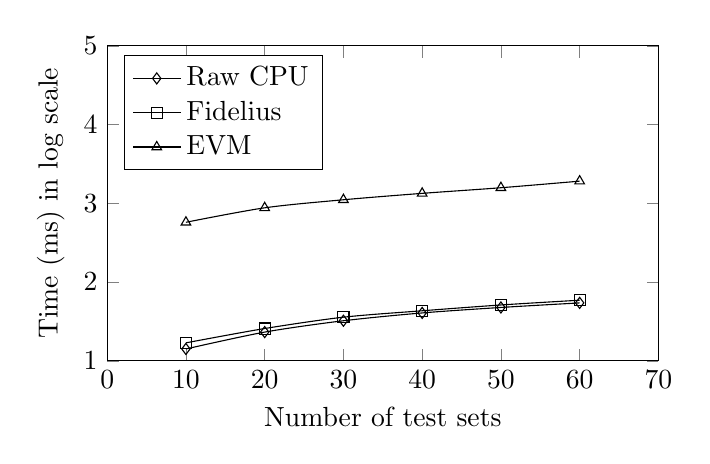
\begin{tikzpicture}
    
\pgfplotsset{
    scale only axis,
    xmin=0, xmax=70,
    ymin=1, ymax=5,
    compat=newest,
    legend pos=north west,
}

\begin{axis}[
  %axis y line*=left,
  %scaled y ticks=base 10:2,
  x=0.1cm,
  y=1cm,
  xlabel=Number of test sets,
  %width=0.4\textwidth,
  %height=0.6\textwidth,
  ylabel=Time (ms) in log scale,
]

\addplot[smooth,mark=diamond]
  coordinates{
    (10,1.1501) %log10(14.13)
    (20,1.3642) %log10(23.13)
    (30,1.5083) %log10(32.23)
    (40,1.6076) %log10(40.51)
    (50,1.6771) %log10(47.54)
    (60,1.7350) %log10(54.32)
}; \label{plot_raw}

\addplot[smooth,mark=square]
  coordinates{
    (10,1.2276) %log10(16.89)
    (20,1.4096) %log10(25.68)
    (30,1.5535) %log10(35.77)
    (40,1.6350) %log10(43.15)
    (50,1.7088) %log10(51.14)
    (60,1.7693) %log10(58.79)
  }; \label{plot_fid}

\addplot[smooth,mark=triangle]
  coordinates{
    (10,2.7589) %log10(574)
    (20,2.9425) %log10(876)
    (30,3.0449) %log10(1109)
    (40,3.1261) %log10(1337)
    (50,3.1976) %log10(1576)
    (60,3.2813) %log10(1911)
  }; \label{plot_evm}


  \addlegendimage{/pgfplots/refstyle=plot_raw}\addlegendentry[right]{Raw CPU}
  \addlegendimage{/pgfplots/refstyle=plot_fid}\addlegendentry[right]{Fidelius}
  \addlegendimage{/pgfplots/refstyle=plot_evm}\addlegendentry[right]{EVM}

\end{axis}
\end{tikzpicture}
}
  

  \caption{\small Time Consumption on Raw CPU, Fidelius and EVM.}
\label{fig:knn_cmp}
\end{figure}

Figure~\ref{fig:knn_cmp} shows the time consumption of the \textit{k}-NN algorithm on raw CPU, Fidelius, and the Ethereum Virtual Machine (EVM), with the latter taking roughly 30 times longer than the others. Additionally, EVM executions often fail when testing more than 60 sets due to memory constraints, highlighting the difficulties of running complex machine learning algorithms with large datasets on the EVM, as also noted in previous studies about Ethereum's memory limits~\cite{dinh2017blockbench}. In contrast, Fidelius provides a more reliable and stable environment for sophisticated machine learning tasks.

\section{Related Work}\label{sec:related}
GXS~\cite{gxchain} operates as a blockchain-based data trading platform that records and facilitates transactions between buyers and sellers, who exchange data via private channels upon mutual agreement.
AccountTrade~\cite{accounttrade} uses blockchain to pair analyzers with data providers and ensures ecosystem security through enforceable protocols and data indices that detect and penalize dishonest behaviors.
Zhao et al.~\cite{zhao} developed a data trading system focused on provider privacy, employing ring signatures and double authentication to secure transactions and prevent unauthorized access.


In data-sharing systems~\cite{dong2015secure,yue2017big,xia2017medshare}, Shen et al.~\cite{shen} develop a scheme that ensures data integrity and confidentiality.
Zuo et al.~\cite{FG} introduce a system that efficiently safeguards and revokes sellers' secret keys using proxy re-encryption and key separation, enhancing data protection with attribute-based encryption.
To mitigate malicious proxy involvement in data leaks, Guo et al.~\cite{APRE} present accountable proxy re-encryption (APRE), a framework that detects and addresses misuse of re-encryption keys, further validating its CPA security and accountability under the DBDH assumption.
Deng et al.~\cite{IBET} formalize an identity-based encryption transformation (IBET) model for sharing encrypted data with additional recipients beyond the initial designation by the data owner.


SDTE~\cite{dai2019sdte} introduces a blockchain-based data analysis platform where data providers encrypt and upload data to the blockchain. Data users select this data, form analysis contracts, and request services. Upon approval, providers send decryption keys to a trusted node via Intel SGX remote attestation, which then decrypts the data and runs the analysis in the Ethereum Virtual Machine (EVM) protected by Intel SGX, before uploading the results to a settlement contract.
However, SDTE's encrypted data uploads exert significant storage demands on the blockchain, and running analysis as Ethereum smart contracts introduces performance challenges. Running complex algorithms like \textit{k}-NN on the EVM, as shown in Section~\ref{subsec:evm_cmp}, is often impractical due to the scale of data and complexity of tasks.


PrivacyGuard~\cite{xiao2020privacyguard} mitigates the performance limitations of the Ethereum Virtual Machine (EVM) by transitioning on-chain analysis to off-chain Trusted Execution Environments (TEEs), allowing data providers to set policies that limit unauthorized data usage. However, it still encounters challenges with EVM performance. Similarly, Sterling~\cite{hynes2018demonstration} introduces a decentralized data market utilizing machine learning for data analysis but also places significant storage demands on the blockchain, like SDTE and PrivacyGuard. Moreover, privacy concerns or regulations may prevent the upload of sensitive data.
\section{Conclusion}\label{sec:conclude}
%We introduced Fidelius, a novel system designed to enhance the security of data analysis in complex scenarios involving multiple roles. Leveraging Intel SGX and blockchain technology, Fidelius addresses the challenges of data leakage, trustworthiness, and verifiability of computation results. By employing static binary analysis and a privacy description language (PDL), Fidelius prevents data leakage in computation results, while its cryptographic protocol ensures the trustworthiness and verifiability of these results. Additionally, Fidelius utilizes local attestation to achieve consistent verification of analysis programs, reducing reliance on centralized services and improving efficiency. Experimental results demonstrate that Fidelius incurs minimal overhead while outperforming existing solutions. Overall, Fidelius presents a promising approach to enhance the security of data analysis, offering a robust solution for protecting sensitive data in diverse and complex scenarios.
Fidelius is a novel system that enhances data analysis security in complex, multi-role scenarios. Leveraging Intel SGX and blockchain technology, it tackles data leakage and guarantees trustworthy, verifiable computation outcomes. By employing static binary analysis and a privacy description language (PDL), Fidelius secures results while its cryptographic protocol ensures integrity. Local attestation consistently verifies analysis programs, reducing reliance on centralized services and boosting efficiency. Experiments show that Fidelius incurs minimal overhead while outperforming existing solutions, offering a robust approach to protecting sensitive data in diverse environments.

%%
%% The next two lines define the bibliography style to be used, and
%% the bibliography file.
\bibliographystyle{ACM-Reference-Format}
\bibliography{sample-base}


%%
%% If your work has an appendix, this is the place to put it.

\end{document}
\endinput
%%
%% End of file `sample-sigconf.tex'.
